% !Mode:: "TeX:UTF-8"
% !TEX program  = xelatex

%\documentclass{cumcmthesis}
\documentclass[withoutpreface,bwprint]{cumcmthesis} %去掉封面与编号页
\usepackage[framemethod=TikZ]{mdframed}
\usepackage{url}   % 网页链接
\usepackage{subcaption} % 子标题
\title{基于蒙特卡罗方法的穿越沙漠游戏决策模型}
\tihao{B}
\baominghao{202010038016}
\schoolname{南京大学}
\membera{陈万驰 181840033 数学系}
\memberb{姜玉骅 181870080 工程管理学院}
\memberc{佘帅杰 181860077 计算机科学与技术系}
\supervisor{教练组}
\yearinput{2020}
\monthinput{09}
\dayinput{13}

\begin{document}

\maketitle
\begin{abstract}
水和食物是沙漠中重要的生命资源。由于沙漠复杂多变的天气等因素,对如何合理分配资源和行为决策的研究具有深远的意义。
本文针对穿越沙漠这一游戏,利用多种方法对这个问题进行了探究。

首先,本文利用数学语言对游戏过程加以描述,将地图压缩到只包括起点、终点、矿山、村庄四种特殊点,用Dijkstra算法求出各个特殊点之间的最短距离。将复杂的
游戏过程转化为玩家在几个特殊点之间的移动和其他行为(如购买物资,挖矿等行为),从而降低模型复杂度。

针对问题一,本文根据化简得到的两张地图,分析地图特性,规划出了最优路径的解空间,利用有限空间穷举法和蒙特卡洛模拟法,分别得到10430元和12020元的最终资金,以及对应的最优策略。

针对问题二,本文根据第一、二关的先验知识,估算天气概率,随机生成天气序列。结合地图信息和当天天气情况,给出玩家应采取的动态策略。然后利用蒙特卡洛模拟,分别对第三关、第四关进行求解。结果为第三关应直奔终点,最佳预期资金为9450元左右;第四关预期平均收益趋近于10800元。

针对问题三,本文分别对第五关的两种可能的最优策略进行大量模拟,得到两名玩家在不同策略下的期望收益,根据Nash平衡理论,得到两名玩家达到最佳预期收益的混合策略,即以0.654的概率在高温天停留。对于第六关,本文在每一个状态下采用蒙特卡洛动态评估方法对当前的可能行动进行评分,并执行评分最高的行动,最终给出了在有两名玩家干扰情况下的最优策略。

\keywords{蒙特卡罗方法 \quad 纳什平衡 \quad 穷举法}
\end{abstract}


\section{问题重述与分析}
穿越沙漠:玩家凭借一张地图,利用初始资金购买一定数量的水和食物(包括食品和其他日常用品),从起点出发,按照游戏规则在沙漠中行走。途中会遇到不同的天气,也可在矿山、村庄补充资金或资源,目标是在规定时间内到达终点,并保留尽可能多的资金。

游戏原地图较为复杂,但事实上有意义的结点只有起点、终点、村庄和矿山,因此求解时考虑使用Dijkstra\cite{dijkstra},求出这四类结点的最短路径,将原地图压缩到仅包含着四类结点。

下面对各个问题进行讨论与分析
\begin{enumerate}
    \item 对于只有一名玩家并且每天天气全部已知的情况:第一关和第二关必然有确定的最优解,而地图结构并不复杂,因此可以直接通过穷举、蒙特卡罗\cite{mc}等搜索策略求解。

    \item 对于只有一名玩家并且玩家仅知道当天天气的情况:玩家的策略是动态的,解具有随机性,当天策略需结合当天天气和地图参数综合考虑。利用已知的天气数据,用频率估计三种天气出现概率,随机生成天气序列。在问题一的分析与模型的基础上,我们对给定的随机天气进行模拟,并最终得到玩家在第三关和第四关的合适的策略。
    
    \item 对于有多名玩家的情况:玩家之间会相互影响彼此收益和消耗,可以看做一个博弈过程。通过分析和计算可以求出各玩家期望收益达到纳什平衡\cite{nashi}的条件。并给出玩家在游戏中采取的策略。
\end{enumerate}

\section{模型假设}
\begin{enumerate}
    \item 每天的天气情况相互独立。
    \item 玩家每天早上确定策略,晚上完成状态转移及资源、资金结算。
    \item 多人游戏中,各个玩家绝对自私、完全理性。
\end{enumerate}

\section{符号说明}
\begin{table}[H]
    \caption{符号说明表}\label{tab:001} \centering
    \begin{tabular}{ccc}
        \toprule[1.5pt]
        \textbf{参数} & \textbf{定义} & \textbf{单位}\\
        \midrule[1pt]
        $Weight$ & 负重上限 & 千克\\ 
        $Q$ & 初始资金 & 元 \\
        $t$ & 天数 & 天\\
        $m_w$ & 每箱水的质量 & 千克/箱\\
        $m_f$ & 每箱食物的质量 & 千克/箱 \\
        $p_w$ & 水的基准价格 & 元/箱\\
        $p_f$ & 食物的基准价格 & 元/箱\\
        $n_{sw}$ & 晴朗天气下水的基准消耗量 & 箱\\
        $n_{hw}$ & 高温天气下水的基准消耗量 & 箱\\
        $n_{ow}$ & 沙暴天气下水的基准消耗量 & 箱\\
        $n_{sf}$ & 晴朗天气下食物的基准消耗量 & 箱\\
        $n_{hf}$ & 高温天气下食物的基准消耗量 & 箱\\
        $n_{of}$ & 沙暴天气下食物的基准消耗量 & 箱\\
        $P_{t}$ & 第t天开始时玩家所处的位置 & / \\
        $W_{t}$ & 第t天开始时玩家剩余的水 & 箱 \\
        $F_{t}$ & 第t天开始时玩家剩余的食物 & 箱 \\ 
        $Q_{t}$ & 第t天开始时玩家剩余的资金 & 元 \\
        $Q_{Mine}$ & 基础收益 & 元\\
        
        \bottomrule[1.5pt]
    \end{tabular}
\end{table}


\section{模型建立与求解}
\subsection{数学描述}

我们首先将该游戏利用数学语言加以描述。显然该局游戏的最终目的是使玩家到达终点时的收益最大,即
\begin{equation}
	\max Q_{30}+\frac{1}{2}p_wW_{30}+\frac{1}{2}p_fF_{30}
\end{equation}
其中$Q_{t},W_{t},F_{t}$分别表示第t天时玩家所剩下的资金、水和食物量。如果玩家在第30天前到达终点,则其各个属性将会在未来几天视作不变,所以我们以第三十天为统一结束时间。该目标函数有如下约束:
\begin{equation}
	Q_t=Q_{t-1}+Q_{Mine}Mine_t-Shop_t[2p_fShopF_t+2p_wShopW_t]
\end{equation}
其中$$Mine_t=\begin{cases}
0,\quad \text{如果第t天不挖矿}\\
1,\quad \text{如果第t天挖矿}
\end{cases}$$
$$Shop_t=\begin{cases}
0,\quad \text{如果第t天不购物}\\
1,\quad \text{如果第t天购物}
\end{cases}$$
即每天结束时的资金等于前一天的资金加上当天挖矿获得的1000元(如果挖矿的话),再减去在村庄购买食物和水花费的钱(如果购买的话)。其中$ShopF_t$和$ShopW_t$分别表示玩家在第t天购买的食物量和水量(如果购买的话)。
\begin{equation}
F_t=F_{t-1}-2Move_t\triangle F_t-3Mine_tMove_t\triangle F_t-(1-Move_t-Mine_t)\triangle F_t+Shop_tShopF_t
\end{equation}
即每天结束时的食物量等于前一天的食物量减去当天的食物消耗量再加上在村庄购买的食物量(如果购买的话)。
\begin{equation}
W_t=W_{t-1}-2Move_t\triangle W_t-3Mine_t\triangle W_t-(1-Move_t-Mine_t)\triangle W_t+Shop_tShopW_t
\end{equation}
即每天结束时的水量等于前一天的水量减去当天的水消耗量再加上在村庄购买的水量(如果购买的话)。
\begin{equation}
P_{t}=P_{t-1}(1-Move_t)+\bar{P}_{t-1}Move_t
\end{equation}
其中$P_t$表示第t天的位置,$\bar{P_t}$表示第t+1天可以到达的几个相邻区域之一,
$$Move_t=\begin{cases}
1,\quad \text{如果第t天移动}\\
0,\quad \text{如果第t天不移动(包括挖矿、停留)}
\end{cases}$$
\begin{equation}
Shop_t\leqslant If_0[(P_t-C_1)(P_t-C_2)\cdots(P_t-C_n)]
\end{equation}
\begin{equation}
Mine_t\leqslant If_0[(P_{t-1}-K_1)(P_{t-1}-K_2)\cdots(P_{t-1}-K_m)]
\end{equation}其中$C_1,C_2,\cdots,C_n$表示n个村庄的位置,$K_1,K_2,\cdots,K_m$表示m个矿山的位置,
$$If_0(x)=\begin{cases}
1,\quad if\quad x=0\\
0,\quad if\quad x\neq0
\end{cases}$$

$\triangle F$和$\triangle W$分别表示第t天基础消耗的食物量和水量。

\subsection{地图简化}

我们首先引入Dijkstra算法,这是一种在有向赋权图中求两点之间最短路径的高效算法。
\begin{figure}[H]
	\centering
	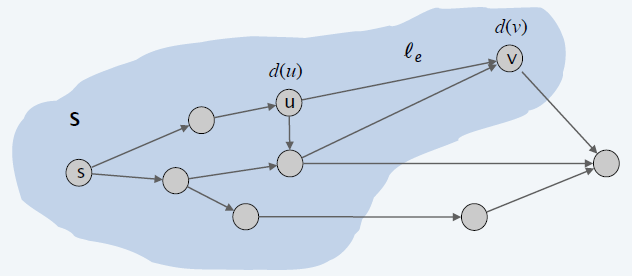
\includegraphics[scale=0.7]{figures/Dijkstra.png}
	\caption{Dijkstra算法示意图}
	\label{fig:Dijkstra}
\end{figure}
如图\ref{fig:Dijkstra},该图中s是起点,最右侧的点是终点。$d(u)$表示从点$s$到点$u$的最短距离。之后执行如下操作:\\
(1)初始化$S={s},d(s)=0$;\\
(2)反复寻找未探索过的点v,使得$\min\quad\pi(v)$,将$v$添加到$S$中,并且$d(v)=\pi(v)$,其中
$$\pi(v)=\min_{e=(u,v):u\in S}d(u)+distance(arg\min_{e=(u,v):u\in S}d(u),v)$$
最终当终点属于$S$时,可以知道起点到终点的最短路径长度,从而问题求解。\\\\
可以看出,问题一的核心关键在于玩家是否前往矿山挖矿、在矿山连续挖几天矿、在挖矿之后是否需要前往村庄补给物资以及是否可以在矿山和村庄之间往返。我们将问题作如下简化:

选取图中起点、终点、村庄和矿山作为特殊点,利用Dijkstra算法计算出每两个特殊点之间的最短路径(即不考虑沙暴天气的影响下,所需最少的天数),如图\ref{fig:map1}所示。

以第一关地图为例,该图每条边上的数字代表着两个特殊点之间的最短路径(不考虑天气影响)。对于问题一,因为天气是预先给定的,整局游戏没有随机因素,所以我们假定玩家在游戏途中始终向着某个特殊点(终点、村庄、矿山)前进并且选择最合适的路径,而非漫无目的地随机移动。
\begin{figure}[H]
	\centering
	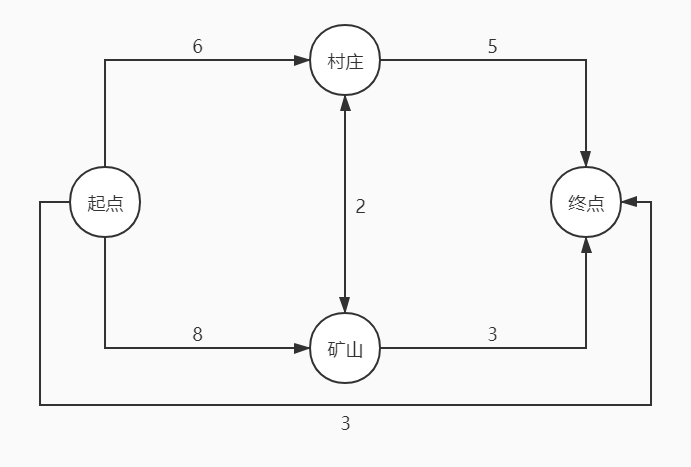
\includegraphics[scale=0.4]{figures/map1newer.jpg}
	\caption{简化后的Map1}
	\label{fig:map1}
\end{figure}

\subsection{问题一}

\subsubsection{第一关}
问题一可简化为玩家在这几个特殊点之间的运动问题。由于第一关地图中村庄在由起点去往矿山的必经之路上,所以应该考虑在玩家第一次到达村庄时适量补充水和食物,然后前往矿山尽可能多地挖矿,在水和食物只够支撑玩家返回村庄时停止挖矿,选择返回村庄。在村庄补给一定量的水和食物(可以通过计算之后几天返回终点时的行程来确定需要购买的水和食物的量,以使得玩家到达终点时水和食物剩余量都为0,从而杜绝资产损失。)


我们将针对第一关的策略方案用流程图的形式展示出来,如图\ref{fig:map1lc}。
\begin{figure}[h]
	\centering
	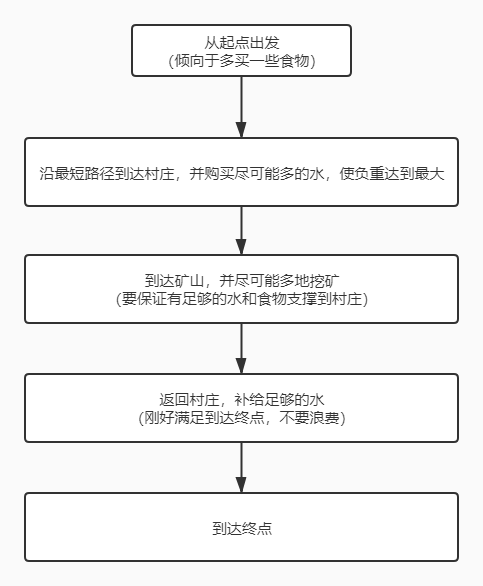
\includegraphics[scale=0.4]{figures/map1liuchengtu}
	\caption{简化的第一关地图}
	\label{fig:map1lc}
\end{figure}
根据这样的流程图,我们进行问题分析和代码求解。玩家在游戏过程中的可选择性因素有:起点处的物资储备、在村庄的物资购买、在矿山挖矿的持续天数、返回村庄时的物资购买等。对此,我们对起点处的物资准备和在矿山挖矿的持续天数进行有范围穷举。对村庄购物策略,基于搜索结果进行调试,以图达到最优。

其中,第一次到达村庄时购买物资的策略为:只购买水,且尽量让负重达到最大。

第二次到达村庄时购买物资的策略为:准确满足之后到达终点所需的全部水和食物,使得到达终点时不剩余任何水和食物。具体代码实现参见附件。\\

经过代码验证,最终找到最佳的策略方案,路径如图\ref{fig:map1word}所示。
\begin{figure}[H]
	\centering
	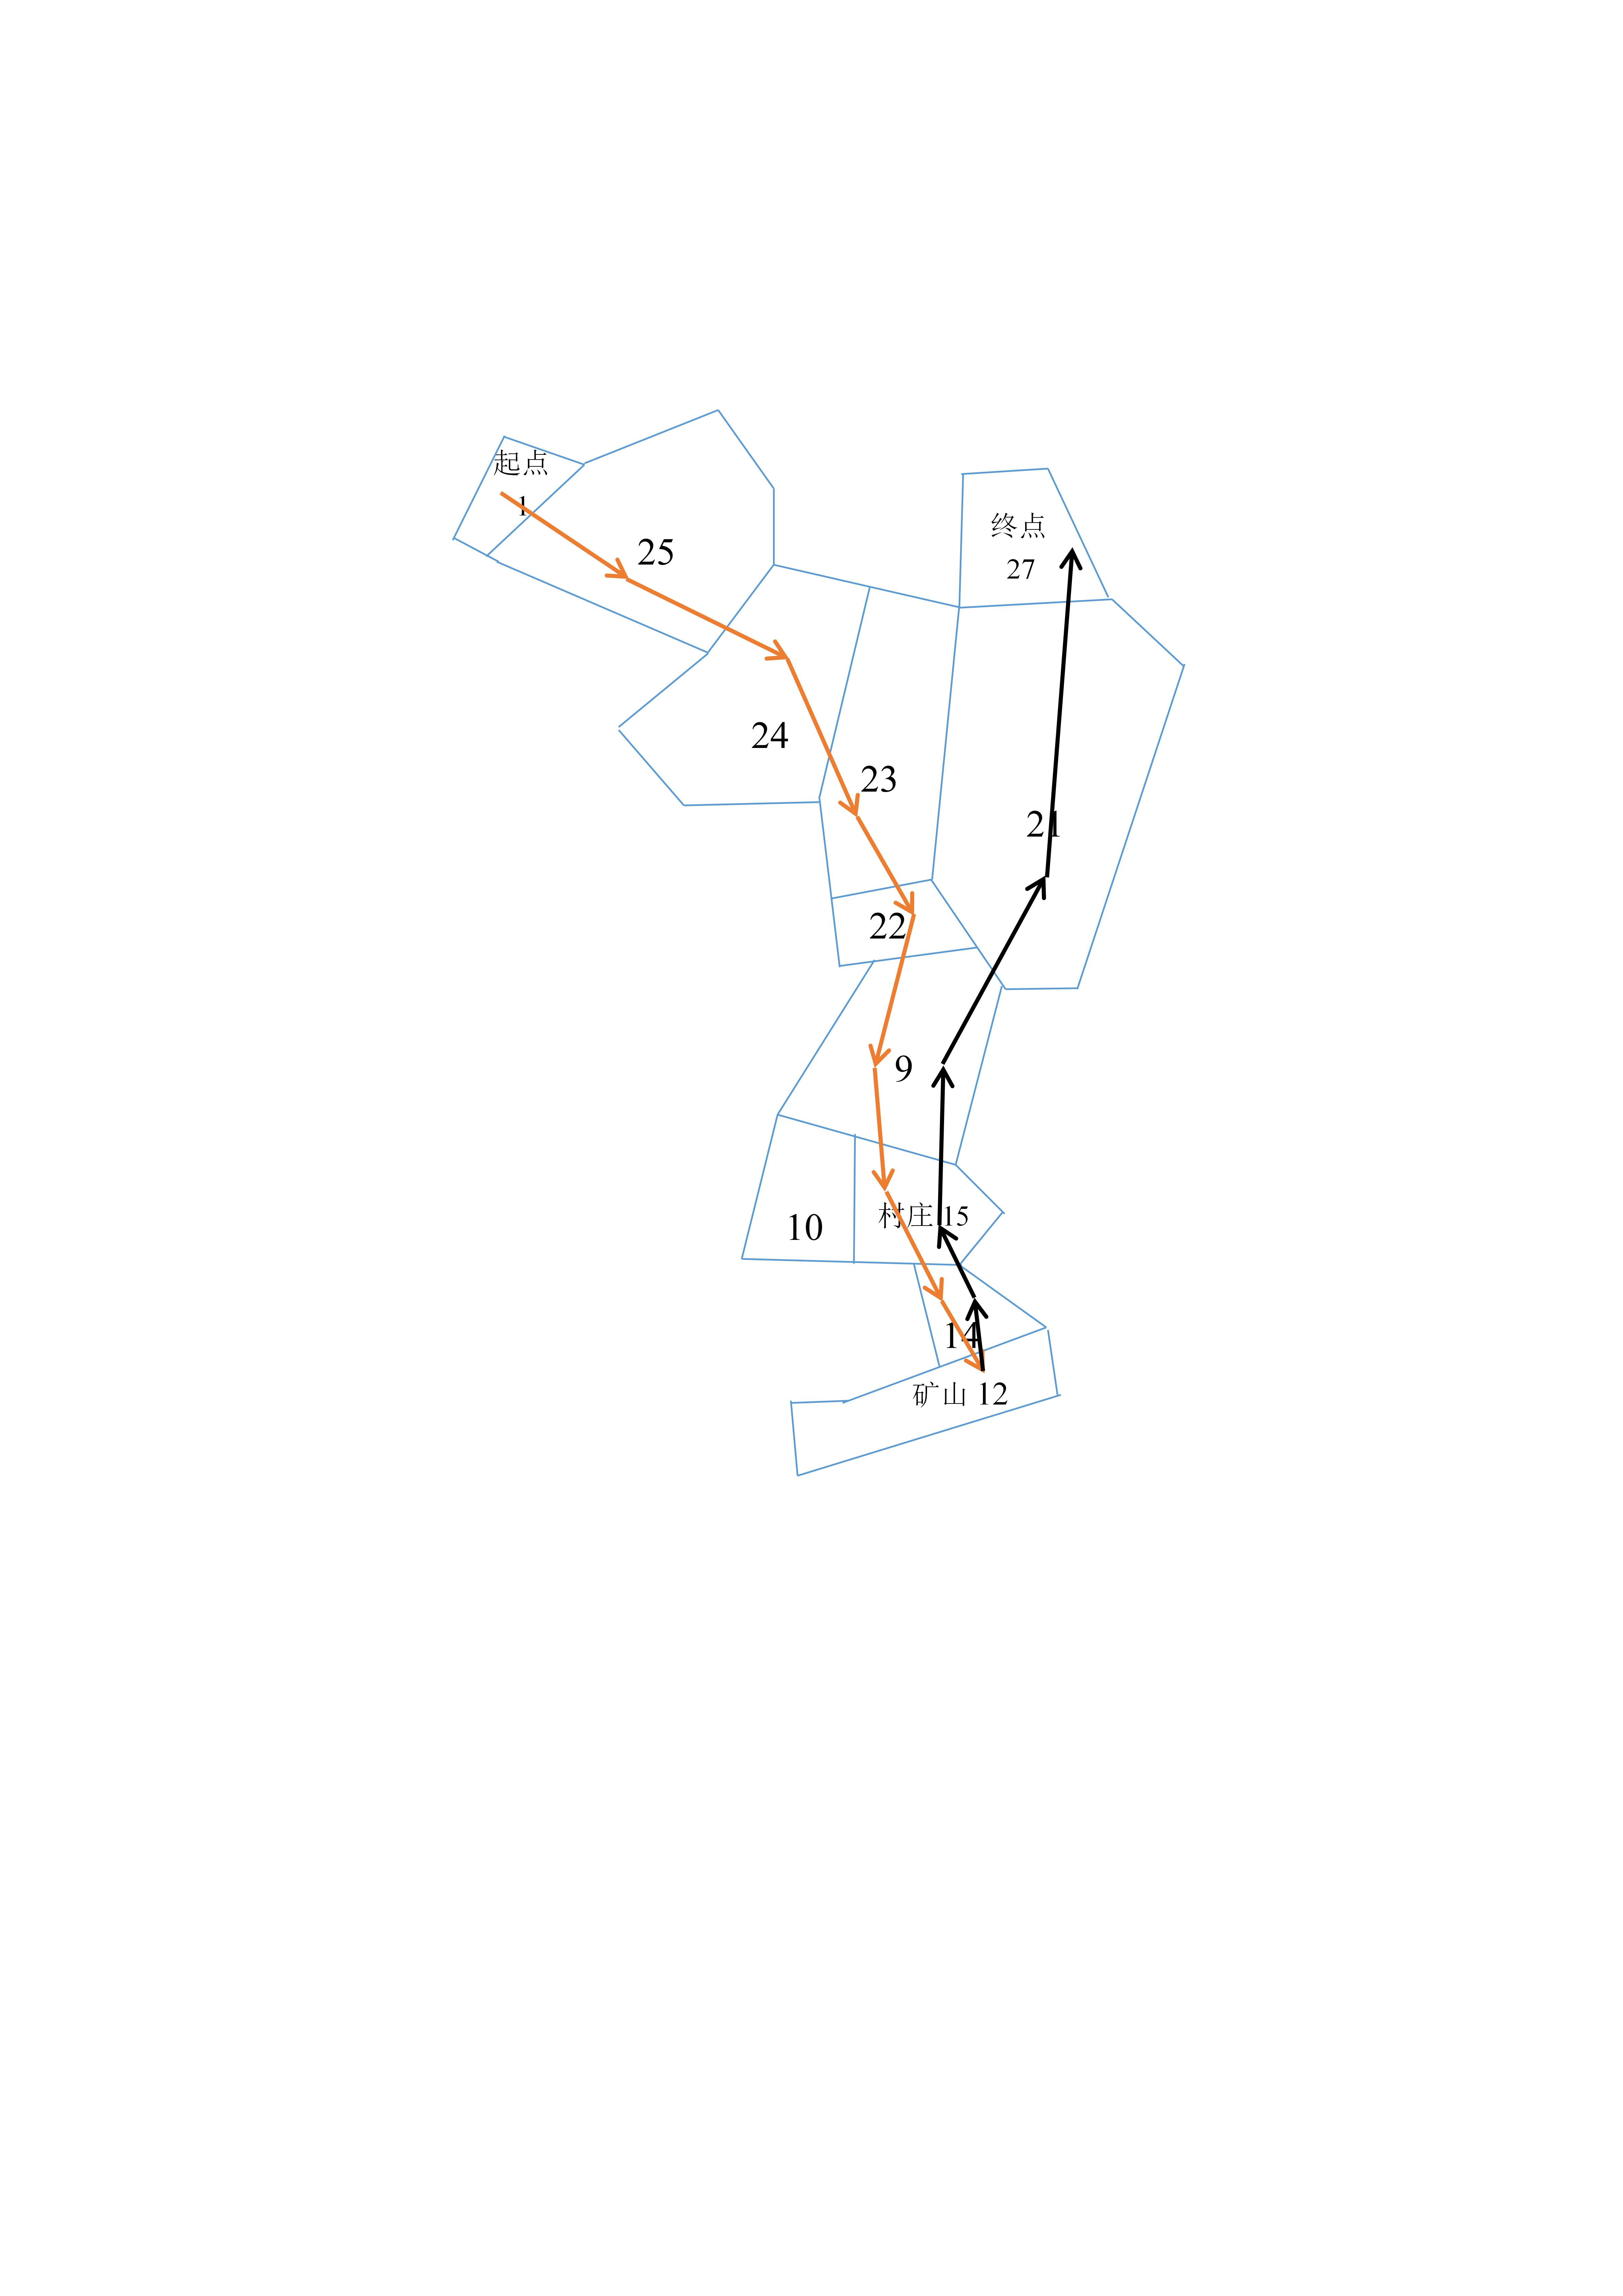
\includegraphics[scale=0.5]{figures/map1word.jpg}
	\caption{第一关路径示意图}
	\label{fig:map1word}
\end{figure}

具体的游戏路径:经历8天时间到达村庄15(其中有2天沙暴天气,只能停在原地),当天在村庄购买水163箱。第二天立即前往矿山,第10天到达矿山,第11-17天进行挖矿,第18天停留在矿山。第19-20天前往村庄,并在第20天当天购买水36箱、食物40箱。第21-23天前往终点,最终于第23天到达终点,水和食物全部消耗完毕。最终剩余资金10430元。完整路径信息参见附件Result.xlsx。

\subsubsection{第二关}
第二关地图较第一关略复杂,包含两个矿山、两个村庄。简化的第二关地图包含6个结点,见\cref{fig:map2}
\begin{figure}[H]
	\centering
	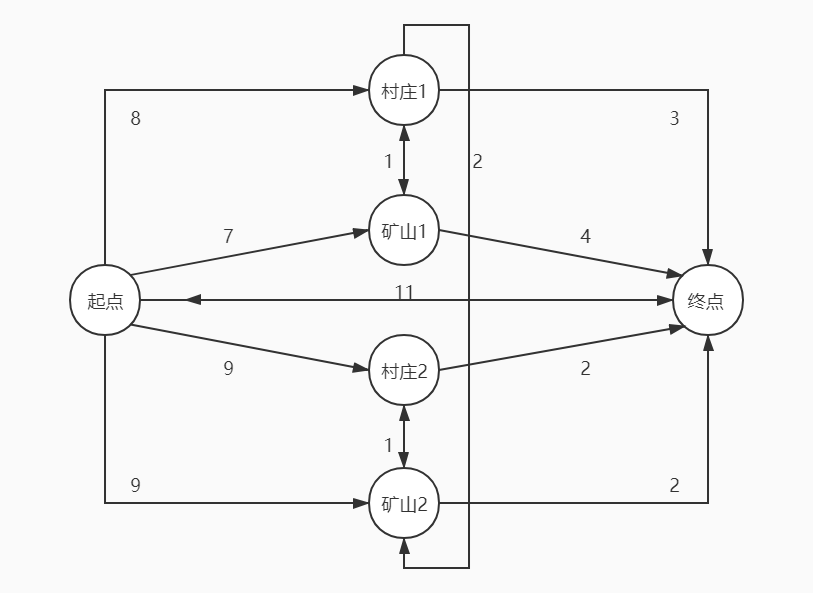
\includegraphics[scale=0.5]{figures/map2.jpg}
	\caption{简化的第二关地图}
	\label{fig:map2}
\end{figure}
由于有范围穷举算法仅仅适合超小规模图,对于第二关这样略大的图,很难寻找到最优解。因此我们采用蒙特卡罗方法对该图进行启发式搜索。启发式搜索过程中,玩家随机在图中进行状态转移,如玩家中途游戏失败则奖励值为0,若玩家在规定时间内成功抵达终点,则奖励值为玩家当前资产加所卖水和食物的钱。

玩家经过村庄尽可能的购买足够多的食物和水,在起点尽可能在不超重情况下购买食物,并保证能够抵达村庄中途补给。具体玩家所购买的食物和水,根据实际情况,进行适当调试以满足实际的搜索需求。

蒙特卡罗搜索的最优奖赏对应的路径见\cref{fig:map2path}
\begin{figure}[H]
	\centering
	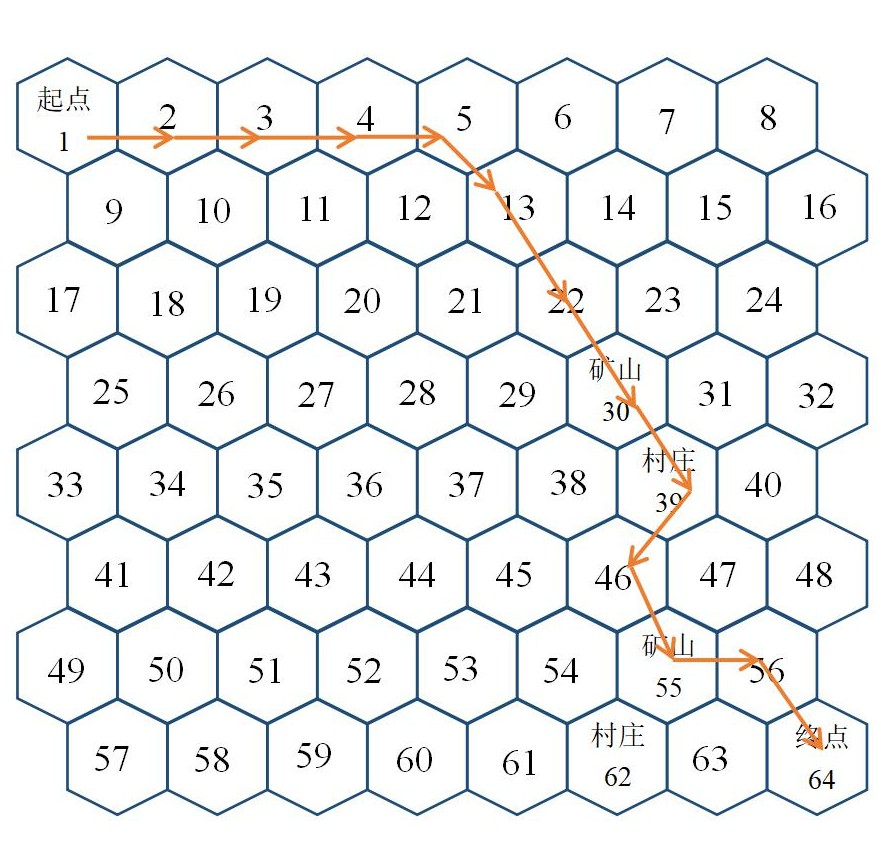
\includegraphics[scale=0.5]{figures/map2path.jpg}
	\caption{第二关最优路径}
	\label{fig:map2path}
\end{figure}

玩家所执行的策略是:从起点以最短路径行走到矿山,于第9天晚上到达(由于沙暴天气延误两天)。挖矿2天后,于第13号晚上到达村庄进行补给。继续行走,于15号晚上到达矿山,挖矿8天后,前往终点,于第24天晚上到达,详细路径信息参见附件Result.xlsx。



\subsection{问题二}


此时玩家仅仅知道当前的天气状况,可据此决定当天的行动方案,即行走或停留或挖矿,整体上的策略仍然分为两种,直接行走到终点或先到矿山挖矿再到终点。玩家可以根据当前天气状况,获取各个行动方案的未来收益,作以下讨论。
\begin{enumerate}
    \item 若玩家不在矿山:
    此时玩家需要决策行走或停留。
    \begin{enumerate}
        \item 沙暴天气必然停留。题目强制要求。
        \item 晴朗天气必然行走。晴朗天气行走消耗资源最少,若晴朗天气不行走,则不存在能够行走的天气状况。
        \item 高温天气需要根据地图参数条件决策。当前时刻为高温,假设下一时刻为晴朗。决策为行走的物资消耗为,水:$2n_{hw}$,食物:$2n_{hf}$。决策为停留等下一时刻晴天再行走的物资消耗为,水:$n_{hw} + 2n_{sw}$,食物:$n_{hf} + 2n_{sf}$。即满足:

        \begin{equation}
            \left\{
                \begin{array}{lr}
                    2n_{sw} < n_{hw}  \\
                    2n_{sf} < n_{hf}
                \end{array}
            \right.
            \label{equa:1}
        \end{equation}
        当前时刻停留的物资消耗更少,因此在时间宽裕的条件下可以考虑在高温天气停留一天。如果当前时刻为高温天气,下一时刻仍为高温天气,另做讨论。
    \end{enumerate}
    \item 若玩家在矿山:此时玩家需要决策行走或停留或挖矿
    \begin{enumerate}
        \item 晴朗天气必然挖矿。晴朗天气挖矿消耗资源最少,若晴朗天气不挖矿,则不存在应挖矿的天气
        \item 高温条件下需要根据地图参数条件决策。决策为挖矿的收益为:$Q_{mine} - 3(n_{hw}p_w + n_{hf}p_f)$,决策为停留的收益为:$-(n_{hw}p_w + n_{hf}p_f)$。即满足下列条件:
        \begin{equation}
            Q_{mine} > 2(n_{hw}p_w + n_{hf}p_f)
            \label{equa:2}
        \end{equation}
        则挖矿收益更高,因此决策为挖矿,否则考虑停留行走。其中$Q_{mine}$为挖矿基本收益,$n_{hw}$、$n{hf}$为高温下水、食物的基本消耗量。以上为考虑当前资源剩余量,若资源剩余量充足,考虑挖矿,若不足,则考虑行走。
        \item 沙暴天气需要根据地图参数条件决策。沙暴天气只能挖矿或停留。决策为挖矿的收益为:$Q_{mine} - 3(n_{ow}p_w + n_{of}p_f)$,决策为停留的收益为:$-(n_{ow}p_w + n_{of}p_f)$。若满足下列条件:
        \begin{equation}
            Q_{mine} < 2(n_{ow}p_w + n_{of}p_f)
            \label{equa:3}
        \end{equation}
        则挖矿收益,因此决策为挖矿,否则停留。其中$n_{ow}$、$n{of}$为沙暴天气下水、食物的基本消耗量。
    \end{enumerate}
\end{enumerate}
由于天气状况未知,因此本题通过蒙特卡罗模拟的方式,寻求玩家动态最佳决策的期望值。实际模拟中,假设每天天气状况相互独立,天气状况可根据第一关、第二关的天气的先验概率分布随机生成,即按2:3:1的概率随机生成晴朗、高温、沙暴三种天气状况。若地图条件满足式\cref{equa:1},即当天为高温天气且下一天为晴朗时,当天选择停留消耗的资源更少。由于存在连续几天出现高温天气的可能性,所以高温天气选择停留可能会产生恶性循环。因此,我们以概率形式表示我们的决策,0.4的概率(下一天为晴天)选择停留,0.6的概率选择行走。

下面就三、四关作具体讨论:
\subsubsection{第三关}
第三关的地图不存在村庄,不存在沙暴天气。因此模型简化了许多。此时玩家路线仅需考虑是直接去终点,还是先经过矿山挖矿再到终点,如\cref{fig:map3}所示。
\begin{figure}[H]
	\centering
	
\includegraphics[scale=0.5]{figures/map3.jpg}
	\caption{简化后的Map3}
	\label{fig:map3}
\end{figure}

第三关地图满足式\cref{equa:1},\cref{equa:2},不满足\cref{equa:3},即玩家的策略如下:
\begin{enumerate}
    \item 晴朗天气:在矿山则挖矿;不在矿山则行走
    \item 高温天气:在矿山不挖矿,0.4概率停留,0.6概率行走;不在矿山0.4概率停留,0.6概率行走。
\end{enumerate}

天气情况按2:3随机生成晴朗、高温。用蒙特卡罗分别对玩家直奔终点和先去矿山再去终点两种路线模拟1000轮,每次模拟100次,取最终资金最高的一次作为本轮最终资金。结果见\cref{fig:check3}
\begin{figure}[H]
    \centering
    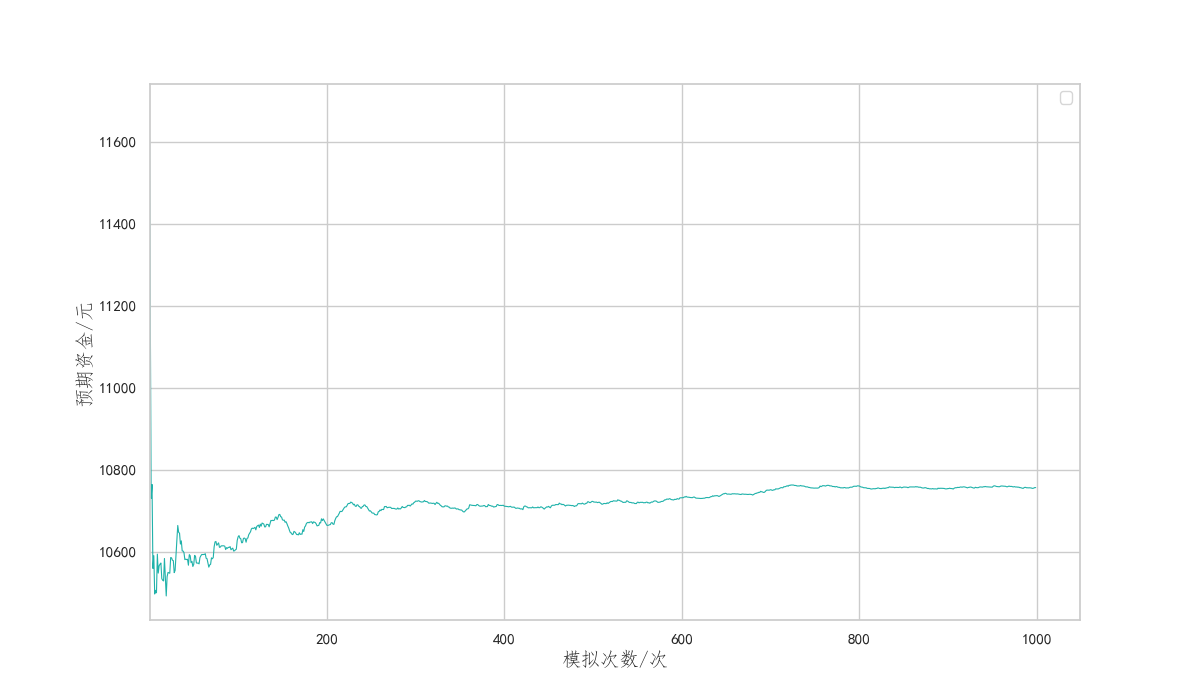
\includegraphics[scale=0.5]{figures/check3.png}
    \caption{第三关蒙特卡罗模拟结果}
    \label{fig:check3}
\end{figure}
可见直接到终点的最佳预期资金稳定在9450元左右,先去矿山再去终点的预期最佳资金稳定在8200元上下。故第三关地图玩家的路线决策应为直奔终点。

\subsubsection{第四关}
第四关的地图有一个村庄、一个矿山且存在沙暴天气。模型较第三关复杂。由于起点到终点的距离等于起点到矿山的距离加上矿山到终点的距离,故玩家必然会挖矿。简化图如\cref{fig:map4}
\begin{figure}[H]
    \centering
    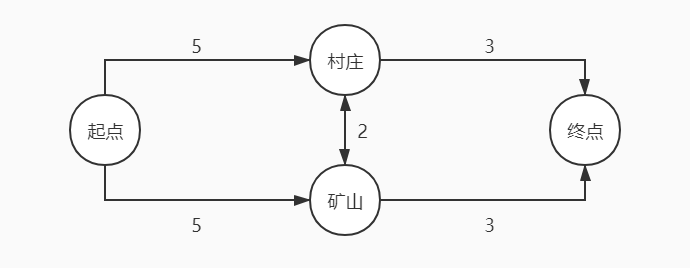
\includegraphics[scale=0.5]{figures/map4.jpg}
    \caption{简化后的Map4}
    \label{fig:map4}
\end{figure}

第四关地图不满足式\cref{equa:1},\cref{equa:2},满足式\cref{equa:3}。即玩家的策略如下:
\begin{enumerate}
    \item 晴朗天气:在矿山则挖矿;不在矿山则行走。
    \item 高温天气:在矿山则挖矿;不在矿山则以0.4概率停留,0.6概率行走。
    \item 沙暴天气:在矿山则挖矿;不在矿山只能停留。
\end{enumerate}
天气情况按2:3:1随机生成晴朗、高温和沙暴。用蒙特卡罗对玩家路线随机模拟1000轮,每轮模拟500次,取最终资金的最高的一次作为本轮的资金。结果见\cref{fig:check4}
\begin{figure}[H]
    \centering
    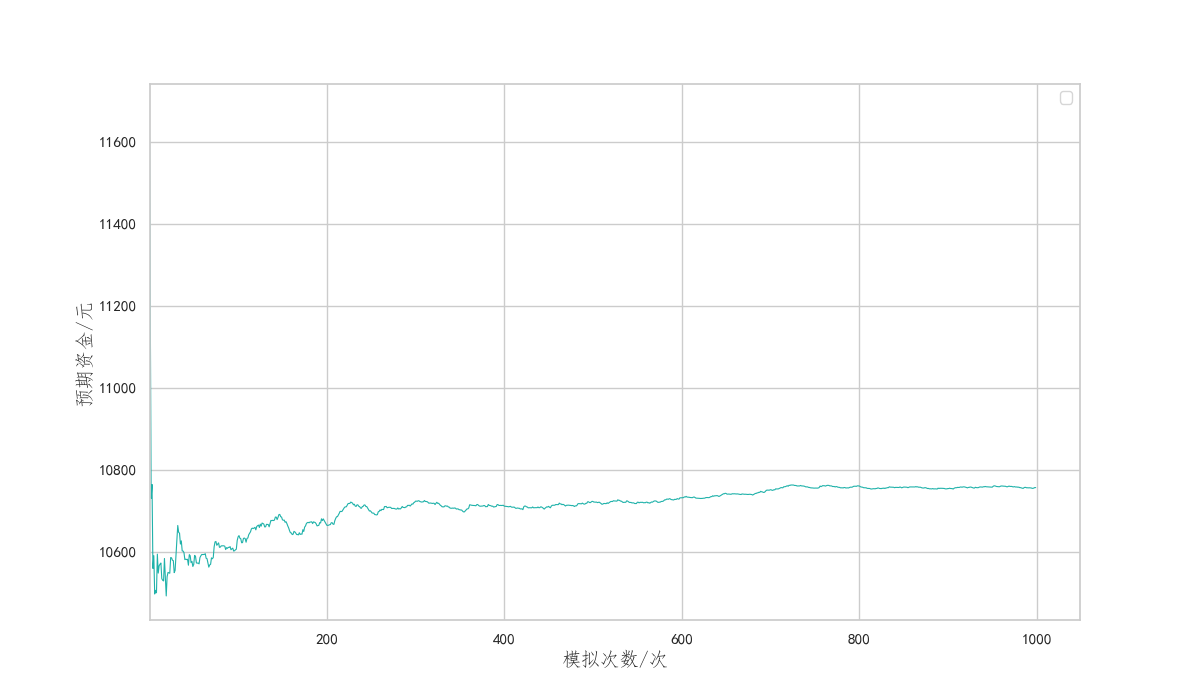
\includegraphics[scale=0.5]{figures/check4.png}
    \caption{第四关蒙特卡罗模拟结果}
    \label{fig:check4}
\end{figure}
可见由于天气带来的随机性,最佳预期资金平均值趋近于10800。
现对于一个表现较好的蒙特卡罗模拟例子作分析。随机生成的天气为[晴朗 , 高温,  高温 ,  高温 ,  晴朗 ,  晴朗 ,  高温 ,  高温 ,  高温 ,  晴朗 ,  高温 ,  晴朗 ,  高温 ,  高温 ,  晴朗 ,  沙暴 ,  沙暴 ,  高温 ,  沙暴 ,  高温 ,  沙暴 ,  沙暴 ,  高温 ,  沙暴 ,  高温 ,  晴朗 ,  沙暴 ,  晴朗 ,  高温 ,  高温]。该天气情况为事实生成的,玩家仍然仅知道当天的天气情况。针对该天气状况,玩家的最优动态策略路径:起点购买240箱水、240箱食物,第5天晚上到达矿山(其中经历沙暴延迟一天),挖矿6天,第13天早上离开,并于16号早上到达终点,最终资金为12590。玩家详细路径如图:
\begin{figure}[H]
	\centering
	
\includegraphics[scale=0.5]{figures/map4path.jpg}
	\caption{一个最优决策路径的图例}
	\label{fig:map4path}
\end{figure}

由于天气因素的随机性以及玩家动态决策的随机性会导致玩家的最佳路径不同、最终资金不同。上述
蒙特卡罗例子只是某种特定情况下的最佳路径,不具有典型代表性。该例子中,玩家不需要经过村庄是因为前期行走过程中天气以晴朗为主,消耗物资较少。若在其它天气情况下,可能需要经过村庄补给。

\subsection{问题三}
\subsubsection{第五关}
第五关的地图较为简单,可简化为如\cref{fig:map5}所示,我们先从单人游戏开始分析。对该图分析可以发现,本关有两种路径:一是直接由起点奔向终点,一是从起点先到矿山,再到终点。第一种路径的最少花费是$(6\times2+18)\times5+(8\times2+18)\times10=150+340=490$。因为天数较少,路径结构较为简单,经过简单计算后发现在第五关地图中,最佳路径是从起点直奔终点,不经过矿山,这样只需实际行走三天。
\begin{figure}[H]
	\centering。
	
\includegraphics[scale=0.5]{figures/map3.jpg}
	\caption{简化后的Map5}
	\label{fig:map5}
\end{figure}
\begin{figure}[H]
	\centering
	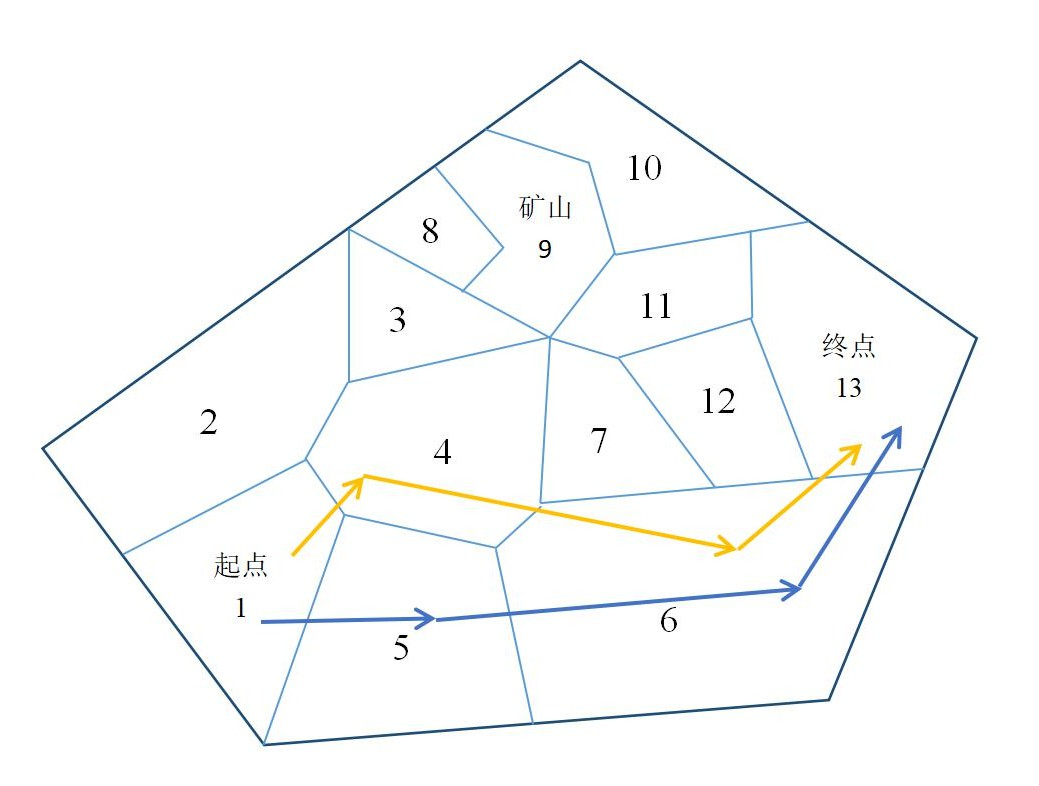
\includegraphics[scale=0.5]{figures/map5path}
	\caption{Map5的两种最优路径}	
\end{figure}
对于二人游戏,由于两名玩家都可以认为是“绝对自私,完全理智”的,所以可以采用静态博弈理论,即两个玩家都知道所有信息(即共同知识),两人同时做出决策,这样的博弈称为完全信息的静态博弈。在该博弈模型中,参与人是两名玩家,每个人的策略空间有两个元素(即是否在高温天停留),每个人的效用函数即是自己最终剩余资金的期望值。

游戏的博弈中参与人集合可以用$N=\{1,2\}$表示,1表示玩家1,2表示玩家2。玩家1的可能的策略记作$a\in A=\{1,2\}$,1、2分别表示选择第2天不停留和停留;玩家2的可能的策略记作$b\in B=\{1,2\}$,1、2分别表示选择第2天不停留和停留。$A$和$B$分别是参与人1和2的策略空间。

对于两名玩家的每一个策略组合$(a,b)$,Map5中都有两种路径,且完全等价,所以我们用计算机进行蒙特卡洛模拟,来计算在该种策略组合下两名玩家的平均收益。用$P(a,b)$和$Q(a,b)$分别表示玩家1和玩家2一次游戏的期望收益,这可以作为玩家1和玩家2的效用函数。经计算得
\begin{equation}
	P=(p_{ij})_{2\times2}=\begin{pmatrix}
	8255.09&8419.88\\8567.58&8402.51
	\end{pmatrix}
\end{equation}
\begin{equation}
    Q=(q_{ij})_{2\times2}=\begin{pmatrix}
    8255.09&8567.44\\
    8420.16&8402.51
    \end{pmatrix}
\end{equation}
可以近似认为$$P=Q'$$

设玩家1采取策略$i$的概率为$p_i(i=1,2)$,玩家2采取策略$j$的概率为$q_j(j=1,2)$,记行向量$\mathbf{p}=(p_1,p_2),\mathbf{q}=(q_1,q_2)$,满足
$$0\leqslant p_i\leqslant1,\quad\sum_{i=1}^{2}p_i=1,\quad0\leqslant q_j\leqslant1,\quad\sum_{j=1}^{2}q_j=1$$
的概率向量分别构成玩家1和玩家2的混合策略空间。

按照混合策略下的Nash均衡理论,计算得
$p_1=q_1=0.346,\quad p_2=q_2=0.654$。
也即玩家1和玩家2应该以34.6\%的概率选择不停留,以65.4\%的概率选择停留。由于两名玩家是完全对称的,所以认为两人所采取的策略应当是完全相同的。我们用蒙特卡洛进行大量模拟两人的游戏过程,通过改变两人选择不停留的概率(两人始终保持概率相同),步长为0.001,最终得到个人的期望收益随概率的变化如图\ref{fig:shouyi}。
\begin{figure}[H]
	\centering
	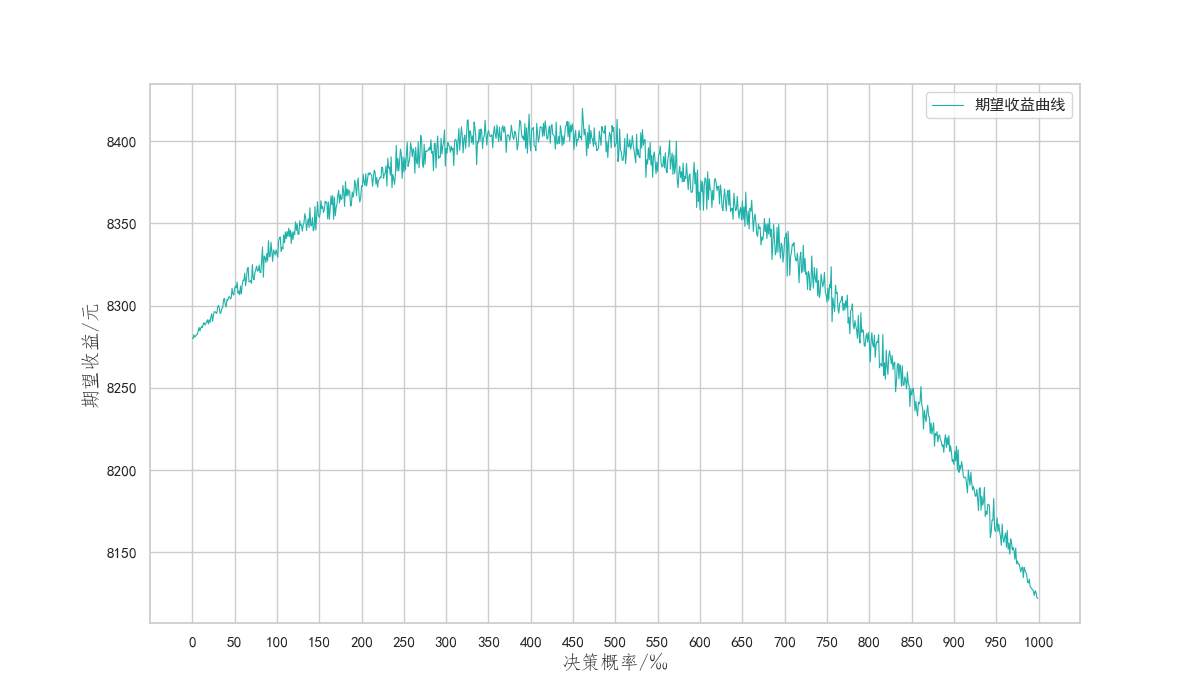
\includegraphics[scale=0.6]{figures/shouyi}
	\caption{个人期望收益随停留概率变化曲线}
	\label{fig:shouyi}
\end{figure}
从图中可以看出,个人期望收益在概率接近0.35到达峰值,这也与我们计算的0.346概率高度吻合,所以可以说明通过混合策略的Nash均衡理论计算出的结果是较为准确可靠的。

\subsection{第六关}
第六关是本题中难度最大的一关,不太可能使用前述算法将可能的情况遍历或模拟,我们用动态评估的方法给出在具体情况下的求解方法。

首先,我们在游戏开始之前,沿用前述方法对天气进行随机模拟,得到天气序列。然后我们使用计算机模拟玩家进行游戏。当玩家走到某一区域时,搜索与该区域相邻的区域作为下一天可采取的行动空间(包括购买物资、采矿等)。之后我们利用蒙特卡洛树搜索方法对这几个区域进行大量模拟,得出几个区域最终的期望收益。即
\begin{equation}
\bar{Q}=\displaystyle\frac{\sum_{i=1}^{n}Q_i}{n}
\end{equation}

其中$\bar{Q}$表示某一区域的期望收益,$Q_i$表示第i次模拟的最终收益。由大数定律可知,当模拟次数足够大时,该区域的期望收益将会收敛于一个值,我们认为该值能代表该区域能给玩家带来的平均收益。所以玩家应在几个可选区域中选取期望收益最高的一个并在下一天执行。

我们以区域17为例来演示这一过程。如图\ref{fig:map6score}所示,区域17周围有四个区域,分别是12、16、18、22,红色数字是各个区域经过大量模拟得到的期望收益,其中16位玩家已走过的区域,12为另外两位玩家(在计算机模拟中固定他们的运动轨迹)要经过的区域,所以这两个区域的期望收益较低;而18是矿场,玩家可以在矿场开采矿石,所以期望收益较高,这也符合实际。最终玩家选择期望收益最高的18区域并在第二天前往到达。


\begin{figure}[H]
	\centering
	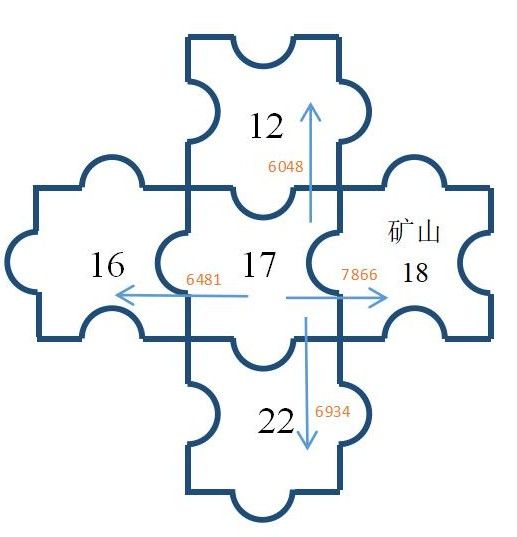
\includegraphics[scale=0.7]{figures/map6score}
	\caption{区域17期望收益计算过程示意图}
	\label{fig:map6score}
\end{figure}

如图\ref{fig:map6path}所示,我们事先给定两个对手玩家(橙色和蓝色)的行动方案,玩家(红色)在每一次行动过后得知机器人的行动方案,并基于这些信息以及前述的期望收益评估方法来规划第二天的行程。最终,玩家路径几乎完美的与其他两个机器人的路径错开。
\begin{figure}[H]
	\centering
	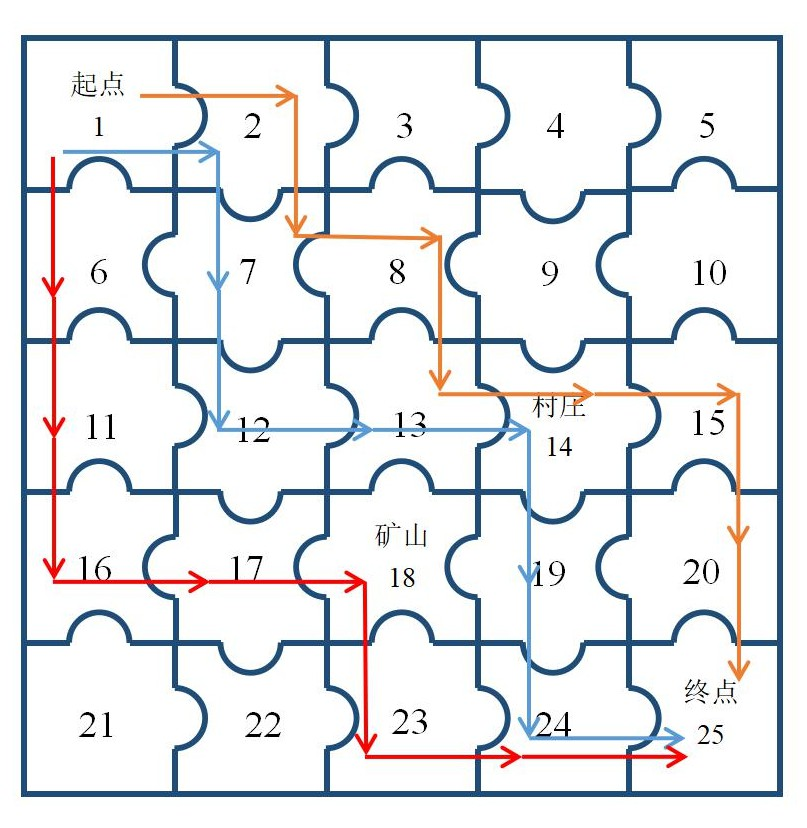
\includegraphics[scale=0.4]{figures/map6path}
	\caption{动态评估给出的玩家最优路径}
	\label{fig:map6path}
\end{figure}
\section{灵敏度分析}
在第三关、第四关模拟中,由于未知天气,原模型中假设晴朗、高温、沙暴天气出现比例为2:3:1,根据这一比例确定了第三关、第四关预期的最终资金。下面我们来分析晴朗、高温、沙暴天气出现比例对第三关、第四关最终资金的灵敏度。

\subsection{第三关}
我们设置5组晴朗、高温天气比例,E1:0.4:0.6;E2:0.45:0.55;E3: 0.5:0.5;E4:0.35:0.65;E5:0.3:0.7
分别用上述天气比例蒙特卡罗模拟第四关100轮,每轮100次,将每轮最终资金的最大值作为该轮的最终资金。分别得到从起点直接去终点的预期最终资金、从起点先到矿山再到终点的预期最终资金,结果见\cref{fig:analysis3map1}、\cref{fig:analysis3map2}。
\begin{figure}[H]
    \centering
    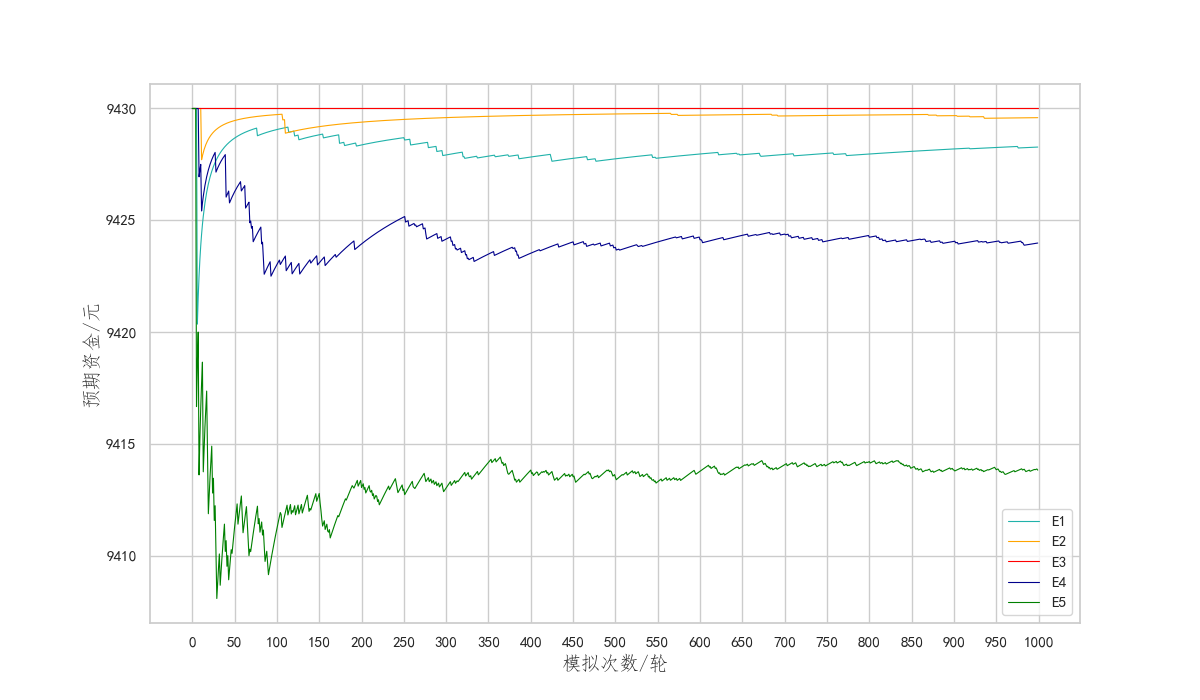
\includegraphics[width=1\textwidth]{figures/analysis3map1.png}
    \caption{第三关:起点到终点预期最终资金}
    \label{fig:analysis3map1}
\end{figure}


\begin{figure}[H]
    \centering
    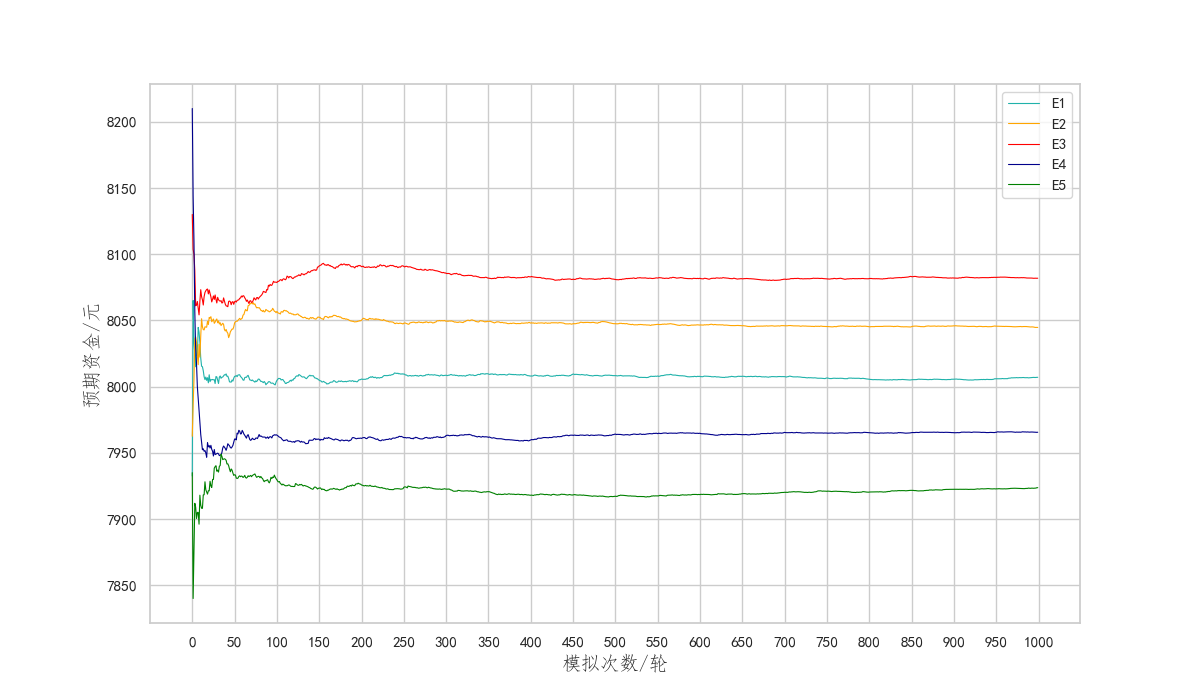
\includegraphics[width=1\textwidth]{figures/analysis3map2.png}
    \caption{第三关:起点到矿山再到终点预期最终资金}
    \label{fig:analysis3map2}
\end{figure}
观察发现,晴朗天气比例的降低或高温天气比例的增高,会导致最终资金的减少。这也正确反映了天气情况对玩家策略、资金的影响。但总的来说,仍然是从起点直接到终点的最终资金比从起点到终点再到矿山的高,验证了我们第三关的结果的正确性。

\subsection{第四关}
我们设置5组晴朗、高温、沙暴天气比例,E1:0.33:0.5:0.17;E2:0.26:0.57:0.17;E3: 0.4:0.43:0.17;E4:0.37:0.5:0.13;E5:0.37:0.53:0.1
分别用上述天气比例蒙特卡罗模拟第四关500轮,每轮500次,将每轮最终资金的最大值作为该轮的最终资金,结果见\cref{fig:analysis4}:
\begin{figure}[H]
    \centering
    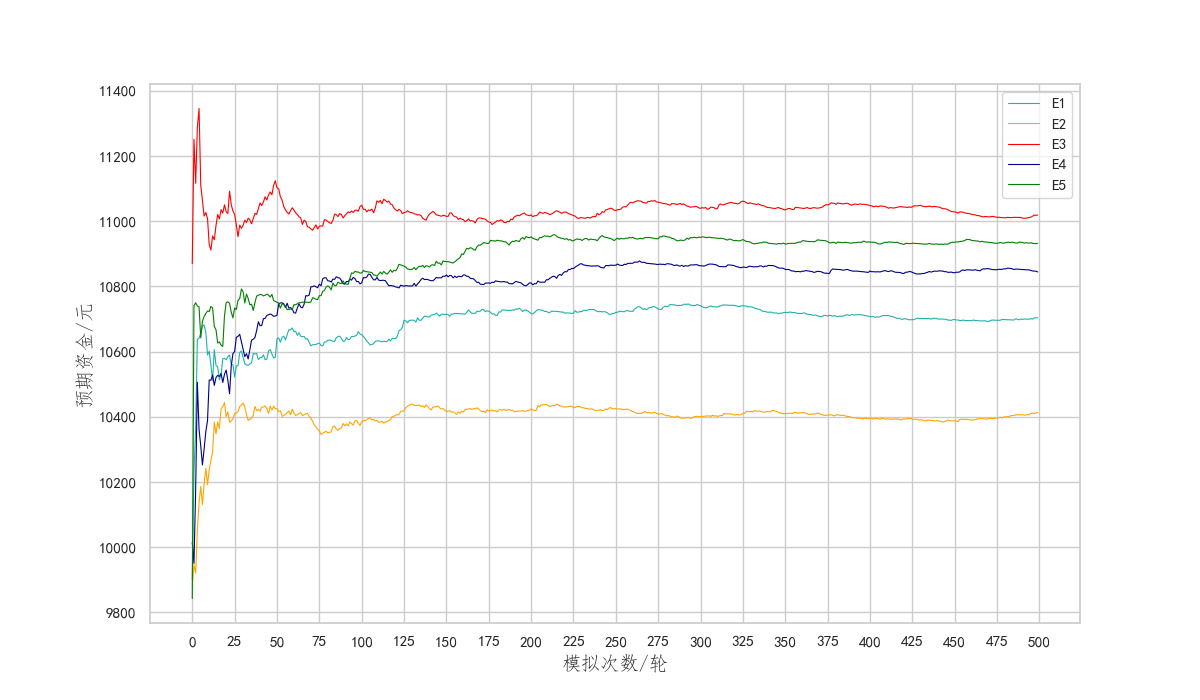
\includegraphics[width=1\textwidth]{figures/anaysis4.png}
    \caption{第四关预期最终资金}
    \label{fig:analysis4}
\end{figure}
观察发现,晴朗天气比例越高、高温和沙暴天气比例越低,会促使最终资金的增加,可见天气随机性对结果会有不小的影响,所以第四关玩家只知道当天的天气,意味着全局最优策略和最高资金也是随机的,与天气情况的随机性息息相关。这样的结果与我们的设想符合。

\section{模型评估}
\subsection{模型优点}
\begin{enumerate}
    \item 将地图图形用矩阵建模,使用地图简化算法,对复杂地图合理简化,极大缩小求解空间,使得原问题变得可解。
    \item 第三题使用Nash理论合理的对博弈过程建模计算,得到稳定的结果
    \item 在模型灵敏度分析中表现稳定,在复杂的多种天气条件下,均可生成较优策略。
    \item 使用动态评估方法评估当前情况的最优解,评估更灵活和准确,可以随时根据条件变化得到贴近值。
\end{enumerate}

\subsection{模型缺点}
\begin{enumerate}
    \item 尽管使用了简化算法,但由于计算影响因子过多导致解空间过大,计算的复杂度难以控制、耗时较长。
    \item 对地图实际情况有一定的依赖,解法不完全具有通用性。
    \item 蒙特卡罗模拟具有一定随机性,求解稳定性有待提高。
\end{enumerate}



%参考文献
\begin{thebibliography}{9}%宽度9
    \bibitem[3]{nashi} 姜启源, 谢金星, 叶俊. 数学模型[M]. 北京: 高等教育出版社, 2003.
    \bibitem[1]{dijkstra} 科曼, Cormen T H. 算法导论[J]. 2006.
    \bibitem[2]{mc} Sutton R S, Barto A G. Introduction to reinforcement learning[M]. Cambridge: MIT press, 1998.

\end{thebibliography}

\newpage
\begin{appendices}
\section{支撑材料文件目录}

% \begin{enumerate}
%     \item Dijkstra\.py
%     \item Draw\.py
%     \item map1\.py
%     \item Map1\.txt
%     \item Map2\.txt
%     \item Map3\.txt
%     \item Map4\.txt
%     \item Map5\.txt
%     \item Map6\.txt
%     \item Map2\_MC\.py 
%     \item Map3\_MC\.py
%     \item Map3\_MC\_Analysis\.py
%     \item Map4\_MC\.py
%     \item Map4\_MC\_Analysis\.py
%     \item Map5\_MC\.py
%     \item Map6\_MC\.py
% \end{enumerate}

















\section{Dijkstra各个点最短路径}
\begin{lstlisting}[language=python]

    # 把地图使用矩阵进行建模
    # 使用图论算法Dijktra算法求解给定点的到其他点的最短距离
    
    def Test(vec,result,v0):
        visit=[]
        last_visit=0
        for i in range(len(vec)):
            visit.append(0)
        visit[v0]=1
        result[0]=0
    
        for i in range(len(vec)):
            for j in range(len(vec)):
    
                if visit[j]==0:
                    dist=vec[v0][j]+last_visit
                    if dist<result[j]:
                        result[j]=dist
            minIndex=0
            while visit[minIndex]==1:
                if minIndex==len(visit)-1:
                    break
                minIndex+=1
            for j in range(minIndex,len(vec)):
                if visit[j]==0 and result[j]<result[minIndex]:
                    minIndex=j
            last_visit=result[minIndex]
            visit[minIndex]=1
            v0=minIndex
    
    Map=[]
    
    class Node:
        def __init__(self,id,state,nodes):
            self.id=id
            self.state=state
            self.neibor=[]
            for i in nodes:
                self.neibor.append(i)
    
    # 这个函数用于建立地图
    def build_map():
        fp = open("Map1.txt",'r') # 根据所求地图修改路径
        node_id=1
        for i in fp:
            if i !=None:
                i=i.split()
                temp_state=i[0]
                temp_list=[]
                for j in range(1,len(i)):
                    temp_list.append(int(i[j]))
                temp_node=Node(node_id,temp_state,temp_list)
                Map.append(temp_node)
                node_id+=1
    
    # 功能算法
    def Dijktra(start: int, mgraph: list) -> list:
        passed = [start]
        nopass = [x for x in range(len(mgraph)) if x != start]
        dis = mgraph[start]
    
        while len(nopass):
            idx = nopass[0]
            for i in nopass:
                if dis[i] < dis[idx]: idx = i
    
            nopass.remove(idx)
            passed.append(idx)
    
            for i in nopass:
                if dis[idx] + mgraph[idx][i] < dis[i]: dis[i] = dis[idx] + mgraph[idx][i]
        return dis
    
    def run():
        n=27
        vec=[]
        # 这里的n和27都是顶点的数目
        result=[]
        for i in range(27):
            result.append(100000000)# 是使用一个无穷大的值进行填充
        for i in range(27):
            temp=[]
            for j in range(27):
                temp.append(100000000000)
            vec.append(temp)
    
        build_map()
        for i in Map:
            for j in i.neibor:
                vec[i.id-1][j-1]=1
    
        #print(vec)
        print(Dijktra(0,vec))
    
    run()
\end{lstlisting}

\section{绘图代码包}
\begin{lstlisting}[language=python]
    import numpy as np
    import matplotlib.pyplot as plt
    from matplotlib.pyplot import MultipleLocator
    import seaborn as sns
    from matplotlib.font_manager import FontProperties
    
    #{darkgrid, whitegrid, dark, white, ticks}
    #{deep, muted, bright, pastel, dark, colorblind}
    sns.set(context='notebook', style='whitegrid', palette='colorblind', font='sans-serif', font_scale=1, color_codes=False, rc=None)
    
    plt.rcParams['font.sans-serif']=['SimHei'] #用来正常显示中文标签
    plt.rcParams['axes.unicode_minus']=False #用来正常显示负号
    #families=[ 'fantasy','Tahoma', 'monospace','Times New Roman']
    
    def Draw(Lines,Names,index,Title,Colors=None):
        if Colors==None:
            Colors=['lightseagreen','orange','red','darkblue','green' ]
        plt.rcParams['figure.figsize'] = (12.0, 7.0)
        for i in range(len(Lines)):
            plt.plot(index,Lines[i],Colors[i],label=Names[i],linewidth=0.8)
    
        English=0
        if English:
            Title_font = {'family': 'fantasy', 'size': 20}
        else:
            Title_font = {'family': "STXinwei", 'size': 20}
        plt.title(Title, Title_font)
    
        if English:
            font1 = {'family': 'Tahoma','size': 14}
        else:
            font1 = {'family': "FangSong", 'size': 14}
        plt.xlabel('决策概率/‰', font1)
        plt.ylabel('期望收益/元', font1,rotation=90)
        plt.legend()
    
        show_num=20
        x_len=len(index)/show_num
        x_major_locator = MultipleLocator(x_len)
        ax = plt.gca()
        ax.xaxis.set_major_locator(x_major_locator)
        plt.show()
    
    def test():
        X = np.linspace(-np.pi, np.pi, 256, endpoint=True)
        C,S = np.cos(X), np.sin(X)
        Draw([C,S],['Cos','Sin'],X,"Test")
        DrawLineWithSeaBorn([C,S],['Cos','Sin'],X,"Sin And Cos")
    
    import pandas as pd
    from pandas.plotting import register_matplotlib_converters
    register_matplotlib_converters()
    def DrawLineWithSeaBorn(Lines,Names,index,Title):
        #index = pd.date_range("1 1 2000", periods=100,freq="m", name="date")
        Lines=np.array(Lines)
        Lines=np.transpose(Lines)
        print(Lines[:,1])
        wide_df = pd.DataFrame(Lines, index, Names)
        print(wide_df)
        f, ax = plt.subplots(figsize=(12.0, 7.0))
        ax.set_title(Title, fontsize=22, position=(0.5, 1.05))
        #ax.invert_yaxis()
        ax.set_xlabel('X Label', fontsize=18)
        ax.set_ylabel('Y Label', fontsize=18)
        sns.lineplot(data=wide_df)
        plt.show()
    
    def DrawBarWithSeaBorn(datas,names,title):
        data={}
        for i in range(len(datas)):
            data[names[i]]=datas[i]
        wide_df = pd.DataFrame(data)
        print(wide_df)
        #sns.barplot(x="color",y="age",data=wide_df,hue="gender")
        sns.barplot(x="color", y="age", palette="Set3",data=wide_df)
        plt.show()
    
    
    def test2():
        color = ['green', 'red', 'green', 'blue', 'blue']
        gender = ['男', '女', '女', '男', '男']
        age = [55, 35, 35, 81, 45]
        DrawBarWithSeaBorn([age,color,gender],['age','color','gender'],"Test")
    
    
    '''
    import pandas as pd
    import seaborn as sns
    
    df = pd.DataFrame({'a' : ['a', 'b' , 'b', 'a'], 'b' : [5, 6, 4, 3] })
    
    # horizontal boxplots
    sns.boxplot(x="b", y="a", data=df, orient='h')
    plt.show()
    # vertical boxplots
    sns.boxplot(x="a", y="b", data=df, orient='v')
    plt.show()
    '''
\end{lstlisting}[language=python]

\section{有限范围穷举法求解第一关}
\begin{lstlisting}[language=python]
    init_water=180
    init_food=330
    money=10000-init_food*10-init_water*5
    
    
    weather=["高温","高温","晴朗","沙暴","晴朗",
             "高温","沙暴","晴朗","高温","高温",
             "沙暴","高温","晴朗","高温","高温",
             "高温","沙暴","沙暴","高温","高温",
             "晴朗","晴朗","高温","晴朗","沙暴",
             "高温","晴朗","晴朗","高温","高温"
             ]
    
    base_consume_water=[5,8,10]
    base_consume_food=[7,6,10]
    
    def get_weather(i):
        if i=="高温":
            return 1
        if i=="晴朗":
            return 0
        else:
            return 2
    
    def go(hhday,road):
    
        already_go=0
        consume_water=0
        consume_food=0
        while already_go<road:
            if hhday>30:
                return -1,-1,-1
            if get_weather(weather[hhday-1])!=2:
                #print(hhday,"Day go",weather[hhday])
                consume_food+=base_consume_food[get_weather(weather[hhday-1])]*2
                consume_water+=base_consume_water[get_weather(weather[hhday-1])]*2
                hhday+=1
                already_go+=1
            else:
                #print(hhday, "Day dont go")
                consume_food += base_consume_food[get_weather(weather[hhday-1])]
                consume_water += base_consume_water[get_weather(weather[hhday-1])]
                hhday += 1
        return consume_water,consume_food,hhday
    
    base_water_price=5
    base_water_weight=3
    base_food_price=10
    base_food_weight=2
    
    def possess_c(cur_water,cur_food,cur_money,cur_day,log):
        can_take=1200-cur_water*3-cur_food*2
        #print(can_take)
        #print(cur_money)
        log=log+"At Day "+str(cur_day)+": "+"Reach c water and food "+str(cur_water)+" "+str(cur_food)+"\n"
        i=0
        if cur_day>18:
            # 准备返程 尽可能只携带足以到达终点的物资
            temp_water=max(36,cur_water)
            temp_food=max(40,cur_food)
            i=temp_water-cur_water
            j=temp_food-cur_food
            temp_money = cur_money - i* base_water_price * 2-j*base_food_price*2
        else:
            # 由于起始点倾向于购买性价比更好的食物,所以这里倾向于购买水已装满背包
            i=int(can_take/base_water_weight)
            j=0
            temp_water=cur_water+i
            temp_food=cur_food
            temp_money=cur_money-i*base_water_price*2
    
        newlog=log+"At Day "+str(cur_day)+": "+"Buy water and food "+str(i)+" "+"\n"
        q,w,e=go(cur_day,3)
        temp_water1=temp_water-q
        temp_food1=temp_food-w
        newlog+="At Day "+str(e)+": "+"Move End water and food "+str(temp_water1)+" "+str(temp_food1)+"\n"
        possess_z(temp_water1,temp_food1,temp_money,e,newlog)
    
        newlog = log+"At Day "+str(cur_day)+": "+"Buy water and food "+str(i)+ "\n"
        q, w, e = go(cur_day, 2)
        temp_water2 = temp_water - q
        temp_food2 = temp_food - w
        newlog += "At Day " + str(e) + ": " + "Move Mine water and food " + str(temp_water2) + " " + str(
            temp_food2) + "\n"
        posseess_k(temp_water2, temp_food2, temp_money, e,newlog)
    
    
    log_list={}
    def possess_z(cur_water,cur_food,cur_money,cur_day,log):
        #print("END ",cur_water*5/2+cur_food*10/2+cur_money,cur_day)
        log+="End "+str(cur_day)+" "+str(cur_water*5/2+cur_food*10/2+cur_money)
        if cur_water<0 or cur_food<0:
            return -1
        log_list[log]=cur_water*5/2+cur_food*10/2+cur_money
        return cur_water*5/2+cur_food*10/2+cur_money
    
    def posseess_k(cur_water,cur_food,cur_money,cur_day,log):
        log = log + "At Day " + str(cur_day) + ": " + "Reach M water and food " + str(cur_water) + " " + str(
            cur_food) + "\n"
        water_limit=cur_water/(base_consume_water[get_weather("晴朗")]*3)
        food_limit=cur_food/(base_consume_food[get_weather("晴朗")]*3)
        total_limit=int(min(water_limit,food_limit))
        total_limit=min(total_limit,30-cur_day)
    
        for i in range(1,total_limit+1):
            temp_food=cur_food
            temp_water=cur_water
            temp_day=cur_day
            newlog=log
            temp_money=cur_money
    
            for j in range(1,i+1):
                temp_water=temp_water-base_consume_water[get_weather(weather[cur_day+j-2])]*3
                temp_food=temp_food-base_consume_food[get_weather(weather[cur_day+j-2])]*3
                temp_day+=1
                temp_money+=1000
                newlog+="At Day " + str(temp_day) + ": " + "Dig " + str(j)+" Days "+str(temp_water) + " " + str(
                temp_food) +" " + str(temp_money)+ "\n"
    
    
            q, w, e = go(temp_day, 2)
            if q < 0:
                continue
            temp_water2 = temp_water - q
            temp_food2 = temp_food - w
    
            if temp_food2 < 0 or temp_water2 < 0:
                continue
            newlog += "At Day " + str(e) + ": " + "Go Village water and food " + str(temp_water2) + " " + str(
                temp_food2) + "\n"
            possess_c(temp_water2, temp_food2, temp_money, e, newlog)
    
            q,w,e=go(temp_day,5)
            if q<0:
                continue
            temp_water1=temp_water-q
            temp_food1=temp_food-w
    
    
            if temp_food1<0 or temp_water1<0:
                continue
    
            newlog += "At Day " + str(e) + ": " + "Go end water and food " + str(temp_water1) + " " + str(
                temp_food1) + "\n"
            possess_z(temp_water1,temp_food1,temp_money,e,newlog)
    
    
    def check(i,j):
        if 3*i+2*j>1200 or 5*i+10*j>10000:
            return False
        else:
            return True
    
    def train():
        i=0
        for init_water in range(150,200):
            for init_food in range(300,360):
                i+=1
                if check(init_water, init_food):
                    q,w,e=go(1,6)
                    log=""
                    possess_c(init_water-q,init_food-w,money,e,log)
        print(i)
    train()
    max=-1
    max_index=0
    for i in log_list:
        if log_list[i]>max:
            max=log_list[i]
            max_index=i
    print(max_index)
    
    import matplotlib.pyplot as plt
    
    index=0
    x=[]
    y=[]
    for i in log_list:
        x.append(index)
        index+=1
        y.append(log_list[i])
    
    plt.scatter(x, y, alpha=0.6)
    plt.show()
\end{lstlisting}[language=python]

\section{蒙特卡罗求解第二关}
\begin{lstlisting}[language=python]
    import numpy as np
    from Draw import Draw
    
    map1 = np.array([[-1,7,9,8,9,-1],
                    [-1,1,-1,1,-1,-1],
                    [-1,-1,1,-1,1,2],
                    [-1,-1,2,-1,-1,-1],
                    [-1,-1,1,-1,-1,2],
                    [-1,-1,-1,-1,-1,0]])
    
    states_list = []
    
    M=1200 # 最大负重
    init_money=10000
    base_water_price=5
    base_water_weight=3
    base_food_price=10
    base_food_weight=2
    
    base_consume_water=[5,8,10]
    base_consume_food=[7,6,10]
    
    # 晴朗 高温 沙暴
    weather=["0","高温","高温","晴朗","沙暴","晴朗",
             "高温","沙暴","晴朗","高温","高温",
             "沙暴","高温","晴朗","高温","高温",
             "高温","沙暴","沙暴","高温","高温",
             "晴朗","晴朗","高温","晴朗","沙暴",
             "高温","晴朗","晴朗","高温","高温"
             ]
    
    def cost(cur_time, cur_state, next_state, cur_water,cur_food,states):
        T = map1[cur_state][next_state]
        last_time = cur_time + T
        t = cur_time
        if(t>30):
            cur_water = -10000000
            cur_food = -10000000
            states.append('die')
            return (last_time, cur_water,cur_food)
        if (cur_state == 1 and next_state == 1) or (cur_state == 2 and next_state == 2): # 挖矿
            if(weather[t] == '晴朗'):
                cur_water -= base_consume_water[0]*3
                cur_food -= base_consume_food[0]*3
            elif(weather[t] == '高温'):
                cur_water -= base_consume_water[1]*3
                cur_food -= base_consume_food[1]*3
            elif(weather[t] == '沙暴'):
                cur_water -= base_consume_water[2]*3
                cur_food -= base_consume_food[2]*3
    
    
        elif(cur_state == next_state): #原地停留
            if(weather[t] == '晴朗'):
                cur_water -= base_consume_water[0]
                cur_food -= base_consume_food[0]
            elif(weather[t] == '高温'):
                cur_water -= base_consume_water[1]
                cur_food -= base_consume_food[1]
            elif(weather[t] == '沙暴'):
                cur_water -= base_consume_water[2]
                cur_food -= base_consume_food[2]
    
        else:  # 行走
            while(t < last_time):
                if(t >30):
                    break
                if(weather[t] == '晴朗'):
                    cur_water -= base_consume_water[0]*2
                    cur_food -= base_consume_food[0]*2
                elif(weather[t] == '高温'):
                    cur_water -= base_consume_water[1]*2
                    cur_food -= base_consume_food[1]*2
                elif(weather[t] == '沙暴'):
                    cur_water -= base_consume_water[2]
                    cur_food -= base_consume_food[2]
                    last_time += 1
                t += 1
            if(t>30):
                cur_water = -10000000
                cur_food = -10000000
                states.append('die')
                
        return (last_time, cur_water,cur_food)
    
    
    def MC(cur_time, cur_state, cur_money, cur_water, cur_food,states):
    
        states.append((cur_time,cur_state,cur_money,cur_water,cur_food))
        if cur_water < 0 or cur_food < 0:
            states_list.append(states)
            return 0
    
        if cur_money < 0:
            states_list.append(states)
            return 0        
    
        if cur_time > 30:
            #print(states)
            states_list.append(states)
            return 0
        
    
        if cur_state == 5: # 终点
            states_list.append(states)
            return cur_money+cur_food*base_food_price/2+cur_water*base_water_price/2
        
        if cur_state == 4 : # 村庄  买东西
            wmax=240
            fmax=240
            if(cur_water < wmax):
                cur_money -= (wmax-cur_water)* base_water_price*2
                cur_water = wmax
            if(cur_food < fmax):
                cur_money -= (fmax-cur_food) * base_food_price*2
                cur_food = fmax
            states.append((cur_time, cur_state, cur_money, cur_water, cur_food))
    
    
        if cur_state == 3: # 买到上限
    
            wmax=238
            fmax=226
            if(cur_water < wmax):
                cur_money -= (wmax-cur_water)* base_water_price*2
                cur_water = wmax
            if(cur_food < fmax):
                cur_money -= (fmax-cur_food) * base_food_price*2
                cur_food = fmax
            states.append((cur_time, cur_state, cur_money, cur_water, cur_food))
    
    
    
        next_state = np.random.choice(len(map1))
        while map1[cur_state][next_state] == -1:
            next_state = np.random.choice(len(map1))
    
    
        (next_time,next_water,next_food) = cost(cur_time,cur_state,next_state,cur_water,cur_food,states)
    
    
        if cur_state == 0:
            return MC(next_time, 
                        next_state, 
                        cur_money, 
                        next_water, 
                        next_food,states)
        if cur_state == 3 or cur_state == 4: # 村庄
            return MC(next_time, 
                next_state, 
                cur_money, 
                next_water, 
                next_food,states)
                    
        if cur_state == 1 or cur_state == 2: # 矿场
            if((cur_state == 1 and next_state == 1) or (cur_state == 2 and next_state == 2)):
                return MC(next_time, 
                        next_state, 
                        cur_money+1000, 
                        next_water, 
                        next_food,states)
            else:
                return MC(next_time, 
                        next_state, 
                        cur_money, 
                        next_water, 
                        next_food,states)
               
    
    
    def Game():
        print('Start')
        iteration = 1000000
        money_list = []
        sum_money = 0
        for i in range(iteration):
            states=[]
            sum_money = MC(1,0,5840,184,324,states)
            money_list.append(sum_money)
        index = np.argmax(money_list)
        print('---index----',index)
        print(max(money_list))
        print('--最优路径--', states_list[index])
    
    Game()
    
\end{lstlisting}[language=python]

\section{蒙特卡罗求解第三关}
\begin{lstlisting}[language=python]
    import numpy as np
    from Draw import Draw
    
    # 直接到达终点
    map1 = np.array([[1,-1,3],
                    [-1,1,2],
                    [-1,-1,0]])
    
    # 先到矿山
    map2 = np.array([[1,3,-1],
                    [-1,1,2],
                    [-1,-1,0]])
    
    states_list = []
    
    M=1200 # 最大负重
    init_money=10000
    base_water_price=5
    base_water_weight=3
    base_food_price=10
    base_food_weight=2
    
    base_consume_water=[3,9,10]
    base_consume_food=[4,9,10]
    
    
    
    
    def cost(cur_time, cur_state, next_state, cur_water,cur_food,states,map_,weather):
        T = map_[cur_state][next_state]
        last_time = cur_time + T
        t = cur_time
        if(t>10):
            cur_water = -10000000
            cur_food = -10000000
            states.append('die')
            return (last_time, cur_water,cur_food)
        if cur_state == 1 and next_state == 1: # 挖矿
            if(weather[t] == 0):
                cur_water -= base_consume_water[0]*3
                cur_food -= base_consume_food[0]*3
            elif(weather[t] == 1):
                cur_water -= base_consume_water[1]*3
                cur_food -= base_consume_food[1]*3
    
    
        elif(cur_state == next_state): #原地停留
            if(weather[t] == 0):
                cur_water -= base_consume_water[0]
                cur_food -= base_consume_food[0]
            elif(weather[t] == 1):
                cur_water -= base_consume_water[1]
                cur_food -= base_consume_food[1]
    
        else:  # 行走
            while(t < last_time):
                if(t >10):
                    break
                if(weather[t] == 0):
                    cur_water -= base_consume_water[0]*2
                    cur_food -= base_consume_food[0]*2
                elif(weather[t] == 1):
                    if(np.random.uniform() < 0.4):
                        cur_water -= base_consume_water[1]
                        cur_food -= base_consume_food[1]
                        last_time += 1
                    else:
                        cur_water -= base_consume_water[1]*2
                        cur_food -= base_consume_food[1]*2
                t += 1
            if(t>10):
                cur_water = -10000000
                cur_food = -10000000
                states.append('die')
                
        return (last_time, cur_water,cur_food)
    
    
    def MC(cur_time, cur_state, cur_money, cur_water, cur_food,states, map_,weather):
    
        states.append((cur_time,cur_state,cur_money,cur_water,cur_food))
        if cur_water < 0 or cur_food < 0:
            states_list.append(states)
            return 0
    
        if cur_money < 0:
            states_list.append(states)
            return 0        
    
        if cur_time > 10:
            states_list.append(states)
            return 0
        
    
        if cur_state == 2: # 终点
            states_list.append(states)
            return cur_money+cur_food*base_food_price/2+cur_water*base_water_price/2
        
        next_state = np.random.choice(len(map_))
        while map_[cur_state][next_state] == -1:
            next_state = np.random.choice(len(map_))
    
        (next_time,next_water,next_food) = cost(cur_time,cur_state,next_state,cur_water,cur_food,states,map_,weather)
    
    
        if cur_state == 0:
            return MC(next_time, 
                        next_state, 
                        cur_money, 
                        next_water, 
                        next_food,states,map_,weather)
                    
        if cur_state == 1: # 矿场
            if(cur_state == 1 and next_state == 1):
                return MC(next_time, 
                        next_state, 
                        cur_money+200, 
                        next_water, 
                        next_food,states,map_,weather)
            else:
                return MC(next_time, 
                        next_state, 
                        cur_money, 
                        next_water, 
                        next_food,states,map_,weather)
               
    
    
    def Game():
        print('Start')
        iteration = 1000
        money_list = []
        returns = []
        E1 = []
        E2 = []
        print('------先到终点-------')
        for k in range(iteration):
            for i in range(100):
                # 0晴朗 1高温 2沙暴
                weather = [-1]
                weather.extend([np.random.choice(np.arange(0,2), p=[0.4,0.6]) for _ in range(10)] )
                states=[]
                sum_money = MC(1,0,9190,54,54,states,map1,weather)
                money_list.append(sum_money)
            returns.append(max(money_list))
            E1.append(sum(returns)/(k+1))
    
        index = np.argmax(money_list)
        print(index)
        print(max(money_list))
        print('--最优路径--', states_list[index])
    
        money_list.clear()
        states_list.clear()
        returns.clear()
        print('------先到矿山-----')
        for k in range(iteration):
            for i in range(100):
                # 0晴朗 1高温 2沙暴
                weather = [-1]
                weather.extend([np.random.choice(np.arange(0,2), p=[0.4,0.6]) for _ in range(10)] )
                states=[]
                sum_money = MC(1,0,6400,240,240,states,map2,weather)
                money_list.append(sum_money)
            returns.append(max(money_list))
            E2.append(sum(returns)/(k+1))
        index = np.argmax(money_list)
        print(max(money_list))
        print('--最优路径--', states_list[index])
        
        # 两种方案比较
        Draw([E1,E2],['直接到终点','先到矿山再到终点'],range(len(E1)),"")
        #Draw([E1],['直接到终点'],range(len(E1)),"MC")
    
    if __name__ == "__main__":
        Game()
    
\end{lstlisting}[language=python]

\section{蒙特卡罗求解第四关}
\begin{lstlisting}[language=python]
    import numpy as np
    from Draw import Draw
    
    map1 = np.array([[-1,5,-1,-1],
                    [-1,1,2,3],
                    [-1,2,1,3],
                    [-1,-1,-1,0]])
    
    states_list = []
    
    M=1200 # 最大负重
    init_money=10000
    base_water_price=5
    base_water_weight=3
    base_food_price=10
    base_food_weight=2
    
    base_consume_water=[3,9,10]
    base_consume_food=[4,9,10]
    
    
    
    
    def cost(cur_time, cur_state, next_state, cur_water,cur_food,states,weather):
        T = map1[cur_state][next_state]
        last_time = cur_time + T
        t = cur_time
        if(t>=30):
            cur_water = -10000000
            cur_food = -10000000
            states.append('die')
            return (last_time, cur_water,cur_food)
        if cur_state == 1 and next_state == 1: # 挖矿
            if(weather[t] == 0):
                cur_water -= base_consume_water[0]*3
                cur_food -= base_consume_food[0]*3
            elif(weather[t] == 1):
                cur_water -= base_consume_water[1]*3
                cur_food -= base_consume_food[1]*3
            elif(weather[t] == 2):
                cur_water -= base_consume_water[2]*3
                cur_food -= base_consume_food[2]*3
    
    
        elif(cur_state == next_state): #原地停留
            if(weather[t] == 0):
                cur_water -= base_consume_water[0]
                cur_food -= base_consume_food[0]
            elif(weather[t] == 1):
                cur_water -= base_consume_water[1]
                cur_food -= base_consume_food[1]
            elif(weather[t] == 2):
                cur_water -= base_consume_water[2]
                cur_food -= base_consume_food[2]
    
        else:  # 行走
            while(t < last_time):
                if(t >30):
                    break
                if(weather[t] == 0):
                    cur_water -= base_consume_water[0]*2
                    cur_food -= base_consume_food[0]*2
                elif(weather[t] == 1): # 高温天气0.4概率停止,0.6概率前行
                    if(np.random.uniform() < 0.4):
                        cur_water -= base_consume_water[1]
                        cur_food -= base_consume_food[1]
                        last_time += 1
                    else:
                        cur_water -= base_consume_water[1]*2
                        cur_food -= base_consume_food[1]*2
                elif(weather[t] == 2):
                    cur_water -= base_consume_water[2]
                    cur_food -= base_consume_food[2]
                    last_time += 1
                t += 1
            if(t>30):
                cur_water = -10000000
                cur_food = -10000000
                states.append('die')
                
        return (last_time, cur_water,cur_food)
    
    
    def MC(cur_time, cur_state, cur_money, cur_water, cur_food,states,weather):
    
        states.append((cur_time,cur_state,cur_money,cur_water,cur_food))
        if cur_water < 0 or cur_food < 0:
            states_list.append(states)
            return 0
    
        if cur_money < 0:
            states_list.append(states)
            return 0        
    
        if cur_time > 30:
            #print(states)
            states_list.append(states)
            return 0
    
        if cur_state == 3: # 终点
    
            states_list.append(states)
            return cur_money+cur_food*base_food_price/2+cur_water*base_water_price/2
    
        if cur_state == 2: # 商店 买到上限
            wmax = min(cur_money / (base_food_price*2 + base_water_price*2),
                        M / (base_food_weight + base_water_weight))
            wmax = int(wmax)
            fmax = wmax
            if(cur_water < wmax):
                cur_money -= (wmax-cur_water)* base_water_price*2
                cur_water = wmax
            if(cur_food < fmax):
                cur_money -= (fmax-cur_food) * base_food_price*2
                cur_food = fmax
    
    
    
        next_state = np.random.choice(len(map1))
        while map1[cur_state][next_state] == -1:
            next_state = np.random.choice(len(map1))
    
        (next_time,next_water,next_food) = cost(cur_time,cur_state,next_state,cur_water,cur_food,states,weather)
    
    
        if cur_state == 0:
            return MC(next_time, 
                        next_state, 
                        cur_money, 
                        next_water, 
                        next_food,states,weather)
    
        if cur_state == 2: # 村庄
            return MC(next_time, 
                next_state, 
                cur_money, 
                next_water, 
                next_food,states,weather)
                    
    
    
        if cur_state == 1: # 矿场
            if(cur_state == 1 and next_state == 1):
                return MC(next_time, 
                        next_state, 
                        cur_money+1000, 
                        next_water, 
                        next_food,states,weather)
            else:
                return MC(next_time, 
                        next_state, 
                        cur_money, 
                        next_water, 
                        next_food,states,weather)
               
    
    
    def Game1():
        #0晴朗 1高温 2沙暴
        # -----------------求单个路径 -----------------
        print('Start')
        iteration = 100000
        money_list = []
        #  states_list = []
        sum_money = 0
        weather = [-1]
        weather.extend([np.random.choice(np.arange(0, 3), p=[1 / 3, 1 / 2, 1 / 6]) for _ in range(30)])
        for i in range(iteration):
            states = []
            sum_money = MC(1, 0, 6400, 240, 240, states, weather)
            money_list.append(sum_money)
        index = np.argmax(money_list)
        print(weather)
        print(index)
        print(max(money_list))
        print('--最优路径--', states_list[index])
        # print(states_list)
        #
        print('Start')
        iteration = 1000
    
    
    
    
    def Game2():
        # ---------------求稳态收敛值-----------------#
        returns = []
        E = []
        sum_money = 0
        for k in range(1000):
            money_list = []
            for i in range(1000):
                states=[]
                weather = [-1]
                weather.extend([np.random.choice(np.arange(0,3),p=[1/3,1/2,1/6]) for _ in range(30)])
                sum_money = MC(1,0,6400,240,240,states,weather)
                money_list.append(sum_money)
            returns.append(max(money_list))
            E.append(sum(returns)/(k+1))
        
    if __name__ == "__main__":
        # 求解单个最优路径
        Game1()
        # 求解多个路径收敛值
        Game2()
    
\end{lstlisting}[language=python]

\section{蒙特卡罗求解第五关}
\begin{lstlisting}[language=python]
    # 本代码模拟了多个玩家根据给定的策略进行运动
    # Lines=[
    #     [1, 4, 3, 9, 11, 13],
    #     [1, 2, 3, 9, 11, 13],
    #     [1, 4, 3, 9, 10, 13],
    #     [1, 2, 3, 9, 10, 13],
    #     [1,5,6,13],
    #     [1,4,6,13]
    # ]
    
    # Lines=[
    #     [1, 4, 3, 9, 11, 13],
    #     [1,5,6,13]
    # ]
    
    Lines=[
        [1,4,6,13],
        [1,5,6,13],
        [1,4,6,13],
        [1,5,6,13]
    ]
    
    # Times=[
    #     [ 1,1,1,0,0,0,1,1,0,0],
    #     [1,1,1]
    # ]
    
    Times=[
        [1,1,1],
        [1,0,1,1]
    ]
    Mines=[0,0,0,1,1,1,0,0,0,0]
    
    weather=[0,1,0,0,0,0,1,1,1,1]
    
    cost=[
        [3,9,10],
        [4,9,10]
    ]
    
    class Player:
        def __init__(self,lineid,cur_time,cur_water,cur_food,cur_money):
            self.lineid=lineid
            self.cur_time=cur_time
            self.cur_water=cur_water
            self.cur_food=cur_food
            self.cur_money=cur_money
            self.point=0
            self.cur_pos = Lines[self.lineid][self.point]
            self.dig=False
            self.go=False
    
        def Policy(self):
            self.cur_pos = Lines[self.lineid][self.point]
            self.dig=False
            self.go=False
            if self.lineid<1:
                if self.cur_time < len(Times[0]):
                    if Times[0][self.cur_time]==1:
                        self.point+=1
                        self.go= True
                    # else:
                    #     if Mines[self.cur_time]==1:
                    #         self.dig=True
                    #         self.cur_money+=200
                    self.cur_time+=1
            else:
                if self.cur_time < len(Times[1]):
                    if Times[1][self.cur_time]==1:
                        self.point+=1
                        self.go = True
                    self.cur_time += 1
        def display(self):
            print(self.lineid," ",self.cur_time," ",self.cur_water," ",self.cur_food," ",self.cur_money," ",self.point," ",self.cur_pos)
    
    def count_loss(pos1,pos2,dig1,dig2,go1,go2,gametime):
        loss1=0
        loss2=0
        if pos1==pos2:
            if dig1==1:
                loss1+=100 #挖矿收益减半
                loss1+=(cost[0][weather[gametime]]*5+cost[1][weather[gametime]]*10)*3
            if dig2==1:
                loss2+=100 #挖矿收益减半
                loss2+=(cost[0][weather[gametime]]*5+cost[1][weather[gametime]]*10)*3
            if go1==1:
                loss1+=(cost[0][weather[gametime]]*5+cost[1][weather[gametime]]*10)*4
            if go2==1:
                loss2+=(cost[0][weather[gametime]]*5+cost[1][weather[gametime]]*10)*4
            if go1==0 and dig1==0:
                loss1+=(cost[0][weather[gametime]] * 5 + cost[1][weather[gametime]] * 10) * 2
            if go2 == 0 and dig2 == 0:
                loss2 += (cost[0][weather[gametime]] * 5 + cost[1][weather[gametime]] * 10) * 2
        else:
            if dig1==1:
                loss1+=(cost[0][weather[gametime]]*5+cost[1][weather[gametime]]*10)*3
            if dig2==1:
                loss2+=(cost[0][weather[gametime]]*5+cost[1][weather[gametime]]*10)*3
            if go1==1:
                loss1+=(cost[0][weather[gametime]]*5+cost[1][weather[gametime]]*10)*2
            if go2==1:
                loss2+=(cost[0][weather[gametime]]*5+cost[1][weather[gametime]]*10)*2
            if go1==0 and dig1==0:
                loss1+=(cost[0][weather[gametime]] * 5 + cost[1][weather[gametime]] * 10)
            if go2 == 0 and dig2 == 0:
                loss2 += (cost[0][weather[gametime]] * 5 + cost[1][weather[gametime]] * 10)
        return loss1,loss2
    
    import random
    
    def Game():
        Score={}
        M=[]
        for i in range(2):
            N=[]
            for j in range(2):
               N.append([0,0])
            M.append(N)
        iter=100000
        for i in range(iter):
            for l in range(2):
                for j in range(2):
                    if l==0:
                        pp1=(random.randint(0, 1))
                    else:
                        pp1=(random.randint(2, 3))
                    if j==0:
                        pp2=(random.randint(0,1))
                    else:
                        pp2=(random.randint(2, 3))
                    p1 = Player(pp1, 0, 42, 47, 9320)
                    p2 = Player(pp2, 0, 42, 47, 9320)
                    loss11=0
                    loss22=0
                    for i in range(5):
                        p1.Policy()
                        p2.Policy()
                        pos1=p1.cur_pos
                        pos2=p2.cur_pos
                        loss1,loss2=count_loss(pos1, pos2, p1.dig, p2.dig, p1.go, p2.go, i)
                        #print("Pos1",pos1,p1.go,loss1," ","Pos2",pos2,p2.go,loss2)
                        loss11+=loss1
                        loss22+=loss2
                    #print(loss11,loss22)
                    #print("\n\n")
                    M[l][j][0]+=(p1.cur_money-loss11)
                    M[l][j][1]+=(p2.cur_money-loss22)
    
    
        for i  in range(2):
            for j in range(2):
                M[i][j][1]=M[i][j][1] / iter
                M[i][j][0] = M[i][j][0] / iter
                print(M[i][j][0],",",M[i][j][1],"      ",end="")
            print("\n")
    
        # for i  in range(5):
        #     for j in range(6):
        #         #print(j[0],",",j[1],"     ",end="")
        #         M[i][j][1]-=M[i+1][j][1]
        #         print(M[i][j][1], end=" ")
        #     print("\n")
    Game()
    from Draw import Draw
    
    def Test():
        Score={}
    
    
        iter=1000
        result=[]
        for point in range(1000):
            s1 = 0
            s2 = 0
            for i in range(iter):
                ret=(random.randint(1, 1000))
                if ret<point:
                    pp1=0
                else:
                    pp1=1
                ret=(random.randint(1, 1000))
                if ret<point:
                    pp2=0
                else:
                    pp2=1
    
                p1 = Player(pp1, 0, 42, 47, 9320)
                p2 = Player(pp2, 0, 42, 47, 9320)
                loss11=0
                loss22=0
                for i in range(5):
                    p1.Policy()
                    p2.Policy()
                    pos1=p1.cur_pos
                    pos2=p2.cur_pos
                    loss1,loss2=count_loss(pos1, pos2, p1.dig, p2.dig, p1.go, p2.go, i)
                    #print("Pos1",pos1,p1.go,loss1," ","Pos2",pos2,p2.go,loss2)
                    loss11+=loss1
                    loss22+=loss2
                    #print(loss11,loss22)
                    #print("\n\n")
                s1+=(p1.cur_money-loss11)
                s2+=(p2.cur_money-loss22)
    
    
            result.append(s1/iter)
    
        Draw([result],["期望收益曲线"],range(len(result)),"")
    Test()
\end{lstlisting}[language=python]

\section{蒙特卡罗求解第六关}
\begin{lstlisting}[language=python]
    Map = []
    Set_strategy=[1,2,7,8,13,14,15,20,25]
    Set_strategy2=[1,2,7,12,13,14,19,24,25]
    class Node:
        def __init__(self, id, state, nodes):
            self.id = id
            self.state = state
            self.neibor = []
            for i in nodes:
                self.neibor.append(i)
    
    
    class Log:
        def __init__(self, time, pos, action, money, water, food):
            self.time = time
            self.pos = pos
            self.action = action
            self.money = money
            self.water = water
            self.food = food
    
        def display(self):
            print("Day: " + str(self.time) + " At: " + str(self.pos) + " Money: " + str(self.money) + " water " + str(
                self.water) + " food " + str(self.food) + " " + self.action)
    
    
    def build_map():
        fp = open("Map6.txt", 'r')
        node_id = 1
        for i in fp:
            if i != None:
                i = i.split()
                temp_state = i[0]
                temp_list = []
                for j in range(1, len(i)):
                    temp_list.append(int(i[j]))
                temp_node = Node(node_id, temp_state, temp_list)
                Map.append(temp_node)
                node_id += 1
    
    
    # 晴朗 高温 沙暴
    import random
    
    weather = ["高温", "高温", "晴朗", "晴朗", "晴朗",
               "高温", "沙暴", "晴朗", "高温", "高温",
               "高温", "高温", "晴朗", "高温", "高温",
               "高温", "晴朗", "晴朗", "高温", "高温",
               "晴朗", "晴朗", "高温", "晴朗", "晴朗",
               "高温", "晴朗", "晴朗", "高温", "高温"
               ]
    
    TotalTake = 1200
    init_money = 10000
    base_water_price = 5
    base_water_weight = 3
    base_food_price = 10
    base_food_weight = 2
    
    base_consume_water = [3, 9, 10]
    base_consume_food = [4, 9, 10]
    
    import random
    
    
    def check(i, j, can_take, canafford):
        use_money = (i * 2 * base_water_price + j * 2 * base_food_price)
        use_weight = (i * base_water_weight + j * base_food_weight)
        if use_money > canafford or use_weight > can_take:
            return False
        else:
            return True
    
    
    # 这个函数作为一个机器人已经决定要从当前位置移动到下一个位置的决策过程
    def Just_Go(cur_time, cur_money, cur_water, cur_food, cur_node,meet):
        if cur_time >= 30:
            return 0
        if weather[cur_time] == "沙暴":
            return MonteCarloRobot(cur_time + 1, cur_money, cur_water - base_consume_water[2],
                                   cur_food - base_consume_food[2], cur_node)
        if weather[cur_time] == "高温":
            neigh = Map[cur_node - 1].neibor
            ret = random.randint(0, len(neigh) - 1)
            return MonteCarloRobot(cur_time + 1, cur_money, cur_water - base_consume_water[1] * 2 * meet,
                                   cur_food - base_consume_food[1] * 2 * meet, neigh[ret])
        if weather[cur_time] == "晴朗":
            neigh = Map[cur_node - 1].neibor
            ret = random.randint(0, len(neigh) - 1)
            return MonteCarloRobot(cur_time + 1, cur_money, cur_water - base_consume_water[0] * 2* meet,
                                   cur_food - base_consume_food[0] * 2* meet, neigh[ret])
        else:
            print("Hit Error !!!!!!!!!!!!!!!!!!")
            exit()
            return
    
    
    def MonteCarloRobot(cur_time, cur_money, cur_water, cur_food, cur_node, last_state=0):
        cur_state = Map[cur_node - 1].state
        if cur_time>=len(Set_strategy):
            Player2_pos=25
            Player3_pos=25
        else:
            Player2_pos=Set_strategy[cur_time]
            Player3_pos=Set_strategy2[cur_time]
        meet=1
        if Player2_pos==cur_node:
            meet+=1
        else:
            if Player3_pos==cur_node:
                meet+=1
        if cur_water < 0 or cur_food < 0:
            # print("No food or water And Dead")
            return 0
        if cur_time > 30:
            # print("Out of Time Dead")
            return 0
        if cur_state == 'z':
            # print("get End point with Money",cur_money+cur_food*base_food_price/2+cur_water*base_water_price/2)
            # return cur_money+cur_food*base_food_price/2+cur_water*base_water_price/2
            return cur_money
        if cur_state == 'p' or cur_state == 's':
            return Just_Go(cur_time, cur_money, cur_water, cur_food, cur_node,meet)
    
        if cur_state == 'k':
            ret = random.randint(0, 2)
            if ret == 0:  # 不挖矿 直接离开
                return Just_Go(cur_time, cur_money, cur_water, cur_food, cur_node,meet)
            else:
                if last_state == 1:
                    temp = MonteCarloRobot(cur_time + 1, cur_money + (1000/meet), cur_water - base_consume_water[0] * 3,
                                           cur_food - base_consume_food[0] * 3, cur_node, 1)
                else:
                    temp = MonteCarloRobot(cur_time + 1, cur_money, cur_water - base_consume_water[0],
                                           cur_food - base_consume_food[0], cur_node, 1)
                # if temp!=0:
                # print("Hit herre")
                # print(temp)
                return temp
    
        if cur_state == 'c':
            cur_take = cur_water * base_water_weight + cur_food * base_food_weight
            can_take = TotalTake - cur_take
            water_can_afford = cur_money / (base_water_price * 2)
            food_can_afford = cur_money / (base_food_price * 2)
            water_can_take = can_take / (base_water_price)
            food_can_take = can_take / (base_food_price)
    
            water_can_buy = int(min(water_can_afford, water_can_take))
            food_can_buy = int(min(food_can_afford, food_can_take))
            if water_can_buy <= 0:
                random_water = 0
            else:
                random_water = random.randint(0, water_can_buy)
            if food_can_buy <= 0:
                random_food = 0
            else:
                random_food = random.randint(0, food_can_buy)
    
            use_money = (random_water * 2 * base_water_price + random_food * 2 * base_food_price)
            use_weight = (random_water * base_water_weight + random_food * base_food_weight)
    
            if use_money > cur_money or use_weight > can_take:
                return Just_Go(cur_time, cur_money, cur_water, cur_food, cur_node,meet)
            else:
                # 带着新买的物资走
                return Just_Go(cur_time, cur_money - use_money, cur_water + random_water, cur_food + random_food, cur_node,meet)
    
    
    from Draw import Draw
    
    Decide_List = []
    
    
    def monte_move(cur_time, cur_money, cur_water, cur_food, cur_node, try_time):
        neigh = Map[cur_node - 1].neibor
        best_score = -1
        best_choice = neigh[0]
    
        for i in neigh:
            Money_sum = 0
            real = 1
            for _ in range(try_time):
                tempmoney = MonteCarloRobot(cur_time + 1, cur_money, cur_water - base_consume_water[0] * 2,
                                            cur_food - base_consume_food[0] * 2, i)
                Money_sum += tempmoney
                if tempmoney != 0:
                    real += 1
            #print(Money_sum)
            Money_sum /= real
    
            if Money_sum > best_score:
                best_choice = i
                best_score = Money_sum
            print("At ", cur_node, " to ", i, " ", Money_sum)
        return best_choice, best_score
    
    
    def monte_dig(cur_time, cur_money, cur_water, cur_food, cur_node, try_time):
        Money_sum = 0
        real = 1
        for _ in range(try_time):
            temp = MonteCarloRobot(cur_time + 1, cur_money + 1000, cur_water - base_consume_water[0] * 3,
                                   cur_food - base_consume_food[0] * 3, cur_node)
            if temp != 0:
                real += 1
            Money_sum += temp
        Money_sum /= real
        return -1, Money_sum
    
    
    def Try_Decide(cur_time, cur_money, cur_water, cur_food, cur_node, Log_list):
        #print("I am in site " + str(cur_node))
        Try_time = 2000
        cur_state = Map[cur_node - 1].state
        if cur_water < 0 or cur_food < 0:
            temp = Log(cur_time, cur_node, "Dead", cur_money, cur_water, cur_food)
            Log_list.append(temp)
            return
        if cur_time >= 30:
            temp = Log(cur_time, cur_node, "Timeout", cur_money, cur_water, cur_food)
            Log_list.append(temp)
            return
    
        if cur_state == 'z':
            temp = Log(cur_time, cur_node, "Reach",
                       cur_money + cur_food * base_food_price / 2 + cur_water * base_water_price / 2, cur_water, cur_food)
            Log_list.append(temp)
            return (cur_time,cur_money + cur_food * base_food_price / 2 + cur_water * base_water_price / 2,0,0,cur_node)
    
        if cur_state == 'p' or cur_state == 's':
            best_choice, best_score = monte_move(cur_time, cur_money, cur_water, cur_food, cur_node, Try_time)
            temp = Log(cur_time, cur_node, "Move" + str(best_choice), cur_money, cur_water, cur_food)
            Log_list.append(temp)
            return (cur_time + 1,cur_money, cur_water - base_consume_water[0] * 2,cur_food - base_consume_food[0] * 2,best_choice)
            # Try_Decide(cur_time + 1, cur_money, cur_water - base_consume_water[0] * 2,
            #                   cur_food - base_consume_food[0] * 2, best_choice, Log_list)
    
        if cur_state == 'k':
            best_choice, best_score = monte_move(cur_time, cur_money, cur_water, cur_food, cur_node, Try_time)
            _, dig_score = monte_dig(cur_time, cur_money, cur_water, cur_food, cur_node, Try_time)
            print("Stay And Dig", dig_score)
            if dig_score > best_score:
                best_choice = -1
                best_score = dig_score
    
            if best_choice == -1:
                temp = Log(cur_time, cur_node, "Dig", cur_money, cur_water, cur_food)
                Log_list.append(temp)
                if len(Log_list) > 2 and Log_list[-2].action == "Dig":
                    return (cur_time + 1, cur_money + 1000, cur_water - base_consume_water[0] * 4,cur_food - base_consume_food[0] * 4, cur_node)
                    # Try_Decide(cur_time + 1, cur_money + 1000, cur_water - base_consume_water[0] * 4,
                    #                   cur_food - base_consume_food[0] * 4, cur_node, Log_list)
                else:
                    return (cur_time + 2, cur_money + 1000, cur_water - base_consume_water[0] * 4,cur_food - base_consume_food[0] * 4, cur_node)
                    # Try_Decide(cur_time + 2, cur_money + 1000, cur_water - base_consume_water[0] * 4,
                    #                   cur_food - base_consume_food[0] * 4, cur_node, Log_list)
            else:
                temp = Log(cur_time, cur_node, "Move" + str(best_choice), cur_money, cur_water, cur_food)
                Log_list.append(temp)
                return (cur_time + 1, cur_money, cur_water - base_consume_water[0] * 2, cur_food - base_consume_food[0] * 2, best_choice)
                # Try_Decide(cur_time + 1, cur_money, cur_water - base_consume_water[0] * 2,
                #                   cur_food - base_consume_food[0] * 2, best_choice, Log_list)
    
        if cur_state == 'c':
            cur_take = cur_water * base_water_weight + cur_food * base_food_weight
            can_take = TotalTake - cur_take
            water_can_afford = cur_money / (base_water_price * 2)
            food_can_afford = cur_money / (base_food_price * 2)
            water_can_take = can_take / (base_water_price)
            food_can_take = can_take / (base_food_price)
    
            water_can_buy = min(water_can_afford, water_can_take)
            food_can_buy = min(food_can_afford, food_can_take)
            best_choice = [0, 0]
            best_score = 0
            for i in range(int(water_can_buy)):
                for j in range(int(food_can_buy)):
                    Money_sum = 0
                    if check(i, j, can_take, cur_money):
                        use_money = (i * 2 * base_water_price + j * 2 * base_food_price)
                        temp_try=int(Try_time/1000)
                        for l in range( temp_try):
                            Money_sum += MonteCarloRobot(cur_time, cur_money - use_money, cur_water, cur_food, cur_node)
                        Money_sum /= Try_time
                        if Money_sum > best_score:
                            best_score = Money_sum
                            best_choice[0] = i
                            best_choice[1] = j
    
            use_money = (best_choice[0] * 2 * base_water_price + best_choice[1] * 2 * base_food_price)
            cur_money -= use_money
            cur_water += best_choice[0]
            cur_food += best_choice[1]
            temp = Log(cur_time, cur_node, "Buy", cur_money, cur_water, cur_food)
            Log_list.append(temp)
    
            best_choice, best_score = monte_move(cur_time, cur_money, cur_water, cur_food, cur_node, Try_time)
            temp = Log(cur_time, cur_node, "Move" + str(best_choice), cur_money, cur_water, cur_food)
            Log_list.append(temp)
            return (cur_time + 1, cur_money, cur_water - base_consume_water[0] * 2, cur_food - base_consume_food[0] * 2, best_choice)
            #Try_Decide(cur_time + 1, cur_money, cur_water - base_consume_water[0] * 2, cur_food - base_consume_food[0] * 2, best_choice, Log_list)
    
    
    def Player(cur_time , cur_money, cur_water, cur_food , cur_node):
        Log_List=[]
        old_state=(cur_time , cur_money, cur_water, cur_food , cur_node)
        while 1:
            # if old_state[4]==25:
            #     break
            new_state=Try_Decide(old_state[0],old_state[1], old_state[2], old_state[3] , old_state[4],Log_List)
            #print(old_state," ",new_state)
            if new_state == None:
                return 0
            if old_state[4]==25:
                break
            old_state=new_state
        for i in Log_List:
            i.display()
        return old_state[1]
    
    
    choose=[ "晴朗", "高温", "沙暴",]
    def init_weather(i,j):
        Sunny=i
        Hot=i+j
        Storm=i+j
        temp_weather=[]
        for i in range(30):
            p=(random.randint(0, 1000))
            choice=0
            if p<Sunny:
                choice=0
            if p>Sunny and p <=Hot:
                choice=1
            if p>Hot:
                choice=2
            temp_weather.append(choose[choice])
        global weather
        weather=temp_weather
    
    def RunGame():
        # T=len(weather)
        # print("Start")
        # Money_sum=0
        # try_time=100000
        # money_list=[]
        # for i in range(try_time):
        #     Money_sum+=MonteCarloRobot(0,2000800,400,1)
        #     money_list.append(Money_sum/(i+1))
        # Draw([money_list], ["测试"], range(len(money_list)), "蒙特卡罗模拟沙漠穿越")
        # print("Average Money",Money_sum/try_time)
        # results=[]
        # result=[]
        # total=0
        # i=0
        # while len(result)!=10:
        #     i+=1
        #     f = 200
        #     w = 200
        #     init_weather(700,250)
        #     rest_money = init_money - (base_food_price * f + base_water_price * w)
        #     temp=Player(0, rest_money, w, f, 1)
        #     if temp==0:
        #         continue
        #     else:
        #         total+=temp
        #         result.append(total/(i))
        #
        # results.append(result)
        #
        # result=[]
        # total=0
        # i=0
        # while len(result)!=10:
        #     i+=1
        #     f = 200
        #     w = 200
        #     init_weather(500,450)
        #     rest_money = init_money - (base_food_price * f + base_water_price * w)
        #     temp = Player(0, rest_money, w, f, 1)
        #     if temp == 0:
        #         continue
        #     else:
        #         total += temp
        #         result.append(total / (i))
        # results.append(result)
        # Draw(results,["0.7+0.25+0.05","0.5+0.45+0.05"],range(len(result)),"不同天气下的决策收益")
        # # for i in best_decide:
        # #     i.display()
        f = 200
        w = 200
        init_weather(700,250)
        rest_money = init_money - (base_food_price * f + base_water_price * w)
        Player(0, rest_money, w, f, 1)
    build_map()
    RunGame()
\end{lstlisting}[language=python]

\section{第三关灵敏度分析}
\begin{lstlisting}[language=python]
    from mc_map3 import *


    # 值
    def analysis1():
        E1 = []
        E2 = []
        E3 = []
        E4 = []
        E5 = []
        # ---------------求稳态收敛值
        print('Start')
        iter1 = 1000
        iter2 = 100
        returns = []
        sum_money = 0
        for k in range(iter1):
            money_list = []
            for i in range(iter2):
                states=[]
                weather = [-1]
                weather.extend([np.random.choice(np.arange(0,2),p=[0.4,0.6]) for _ in range(10)])
                sum_money = MC(1,0,9190,54,54,states,map1,weather)
                money_list.append(sum_money)
            returns.append(max(money_list))
            E1.append(sum(returns)/(k+1))
        
        returns = []
        sum_money = 0
        for k in range(iter1):
            money_list = []
            for i in range(iter2):
                states=[]
                weather = [-1]
                weather.extend([np.random.choice(np.arange(0,2),p=[0.45,0.55]) for _ in range(10)])
                sum_money = MC(1,0,9190,54,54,states,map1,weather)
                money_list.append(sum_money)
            returns.append(max(money_list))
            E2.append(sum(returns)/(k+1))
    
        returns = []
        sum_money = 0
        for k in range(iter1):
            money_list = []
            for i in range(iter2):
                states=[]
                weather = [-1]
                weather.extend([np.random.choice(np.arange(0,2),p=[0.5,0.5]) for _ in range(10)])
                sum_money = MC(1,0,9190,54,54,states,map1,weather)
                money_list.append(sum_money)
            returns.append(max(money_list))
            E3.append(sum(returns)/(k+1))
    
        returns = []
        sum_money = 0
        for k in range(iter1):
            money_list = []
            for i in range(iter2):
                states=[]
                weather = [-1]
                weather.extend([np.random.choice(np.arange(0,2),p=[0.35,0.65]) for _ in range(10)])
                sum_money = MC(1,0,9190,54,54,states,map1,weather)
                money_list.append(sum_money)
            returns.append(max(money_list))
            E4.append(sum(returns)/(k+1))
        returns = []
        sum_money = 0
        for k in range(iter1):
            money_list = []
            for i in range(iter2):
                states=[]
                weather = [-1]
                weather.extend([np.random.choice(np.arange(0,2),p=[0.3,0.7]) for _ in range(10)])
                sum_money = MC(1,0,9190,54,54,states,map1,weather)
                money_list.append(sum_money)
            returns.append(max(money_list))
            E5.append(sum(returns)/(k+1))
    
        Draw([E1,E2,E3,E4,E5],['E1','E2','E3','E4','E5'],range(len(E1)),"")
    
    def analysis2():
        E1 = []
        E2 = []
        E3 = []
        E4 = []
        E5 = []
        # ---------------求稳态收敛值
        print('Start')
        iter1 = 1000
        iter2 = 100
        returns = []
        sum_money = 0
        for k in range(iter1):
            money_list = []
            for i in range(iter2):
                states=[]
                weather = [-1]
                weather.extend([np.random.choice(np.arange(0,2),p=[0.4,0.6]) for _ in range(10)])
                sum_money = MC(1,0,6400,240,240,states,map2,weather)
                money_list.append(sum_money)
            returns.append(max(money_list))
            E1.append(sum(returns)/(k+1))
        
        returns = []
        sum_money = 0
        for k in range(iter1):
            money_list = []
            for i in range(iter2):
                states=[]
                weather = [-1]
                weather.extend([np.random.choice(np.arange(0,2),p=[0.45,0.55]) for _ in range(10)])
                sum_money = MC(1,0,6400,240,240,states,map2,weather)
                money_list.append(sum_money)
            returns.append(max(money_list))
            E2.append(sum(returns)/(k+1))
    
        returns = []
        sum_money = 0
        for k in range(iter1):
            money_list = []
            for i in range(iter2):
                states=[]
                weather = [-1]
                weather.extend([np.random.choice(np.arange(0,2),p=[0.5,0.5]) for _ in range(10)])
                sum_money = MC(1,0,6400,240,240,states,map2,weather)
                money_list.append(sum_money)
            returns.append(max(money_list))
            E3.append(sum(returns)/(k+1))
    
        returns = []
        sum_money = 0
        for k in range(iter1):
            money_list = []
            for i in range(iter2):
                states=[]
                weather = [-1]
                weather.extend([np.random.choice(np.arange(0,2),p=[0.35,0.65]) for _ in range(10)])
                sum_money = MC(1,0,6400,240,240,states,map2,weather)
                money_list.append(sum_money)
            returns.append(max(money_list))
            E4.append(sum(returns)/(k+1))
        returns = []
        sum_money = 0
        for k in range(iter1):
            money_list = []
            for i in range(iter2):
                states=[]
                weather = [-1]
                weather.extend([np.random.choice(np.arange(0,2),p=[0.3,0.7]) for _ in range(10)])
                sum_money = MC(1,0,6400,240,240,states,map2,weather)
                money_list.append(sum_money)
            returns.append(max(money_list))
            E5.append(sum(returns)/(k+1))
    
        Draw([E1,E2,E3,E4,E5],['E1','E2','E3','E4','E5'],range(len(E1)),"")
    
    if __name__ == "__main__":
        # 直奔终点
        analysis1()
        # 先到矿山
        analysis2()    
\end{lstlisting}[language=python]

\section{第四关灵敏度分析}
\begin{lstlisting}[language=python]
    import numpy as np
    from Draw import Draw
    
    map1 = np.array([[-1,5,-1,-1],
                    [-1,1,2,3],
                    [-1,2,1,3],
                    [-1,-1,-1,0]])
    
    states_list = []
    
    M=1200 # 最大负重
    init_money=10000
    base_water_price=5
    base_water_weight=3
    base_food_price=10
    base_food_weight=2
    
    base_consume_water=[3,9,10]
    base_consume_food=[4,9,10]
    
    
    
    
    def cost(cur_time, cur_state, next_state, cur_water,cur_food,states,weather):
        T = map1[cur_state][next_state]
        last_time = cur_time + T
        t = cur_time
        if(t>=30):
            cur_water = -10000000
            cur_food = -10000000
            states.append('die')
            return (last_time, cur_water,cur_food)
        if cur_state == 1 and next_state == 1: # 挖矿
            if(weather[t] == 0):
                cur_water -= base_consume_water[0]*3
                cur_food -= base_consume_food[0]*3
            elif(weather[t] == 1):
                cur_water -= base_consume_water[1]*3
                cur_food -= base_consume_food[1]*3
            elif(weather[t] == 2):
                cur_water -= base_consume_water[2]*3
                cur_food -= base_consume_food[2]*3
    
    
        elif(cur_state == next_state): #原地停留
            if(weather[t] == 0):
                cur_water -= base_consume_water[0]
                cur_food -= base_consume_food[0]
            elif(weather[t] == 1):
                cur_water -= base_consume_water[1]
                cur_food -= base_consume_food[1]
            elif(weather[t] == 2):
                cur_water -= base_consume_water[2]
                cur_food -= base_consume_food[2]
    
        else:  # 行走
            while(t < last_time):
                if(t >30):
                    break
                if(weather[t] == 0):
                    cur_water -= base_consume_water[0]*2
                    cur_food -= base_consume_food[0]*2
                elif(weather[t] == 1): # 高温天气0.4概率停止,0.6概率前行
                    if(np.random.uniform() < 0.4):
                        cur_water -= base_consume_water[1]
                        cur_food -= base_consume_food[1]
                        last_time += 1
                    else:
                        cur_water -= base_consume_water[1]*2
                        cur_food -= base_consume_food[1]*2
                elif(weather[t] == 2):
                    cur_water -= base_consume_water[2]
                    cur_food -= base_consume_food[2]
                    last_time += 1
                t += 1
            if(t>30):
                cur_water = -10000000
                cur_food = -10000000
                states.append('die')
                
        return (last_time, cur_water,cur_food)
    
    
    def MC(cur_time, cur_state, cur_money, cur_water, cur_food,states,weather):
    
        states.append((cur_time,cur_state,cur_money,cur_water,cur_food))
        if cur_water < 0 or cur_food < 0:
            states_list.append(states)
            return 0
    
        if cur_money < 0:
            states_list.append(states)
            return 0        
    
        if cur_time > 30:
            #print(states)
            states_list.append(states)
            return 0
    
        if cur_state == 3: # 终点
    
            states_list.append(states)
            return cur_money+cur_food*base_food_price/2+cur_water*base_water_price/2
    
        if cur_state == 2: # 商店 买到上限
            wmax = min(cur_money / (base_food_price*2 + base_water_price*2),
                        M / (base_food_weight + base_water_weight))
            wmax = int(wmax)
            fmax = wmax
            if(cur_water < wmax):
                cur_money -= (wmax-cur_water)* base_water_price*2
                cur_water = wmax
            if(cur_food < fmax):
                cur_money -= (fmax-cur_food) * base_food_price*2
                cur_food = fmax
    
    
    
        next_state = np.random.choice(len(map1))
        while map1[cur_state][next_state] == -1:
            next_state = np.random.choice(len(map1))
    
        (next_time,next_water,next_food) = cost(cur_time,cur_state,next_state,cur_water,cur_food,states,weather)
    
    
        if cur_state == 0:
            return MC(next_time, 
                        next_state, 
                        cur_money, 
                        next_water, 
                        next_food,states,weather)
    
        if cur_state == 2: # 村庄
            return MC(next_time, 
                next_state, 
                cur_money, 
                next_water, 
                next_food,states,weather)
                    
    
    
        if cur_state == 1: # 矿场
            if(cur_state == 1 and next_state == 1):
                return MC(next_time, 
                        next_state, 
                        cur_money+1000, 
                        next_water, 
                        next_food,states,weather)
            else:
                return MC(next_time, 
                        next_state, 
                        cur_money, 
                        next_water, 
                        next_food,states,weather)
               
    
    
    def Game1():
        #0晴朗 1高温 2沙暴
        # -----------------求单个路径 -----------------
        print('Start')
        iteration = 100000
        money_list = []
        #  states_list = []
        sum_money = 0
        weather = [-1]
        weather.extend([np.random.choice(np.arange(0, 3), p=[1 / 3, 1 / 2, 1 / 6]) for _ in range(30)])
        for i in range(iteration):
            states = []
            sum_money = MC(1, 0, 6400, 240, 240, states, weather)
            money_list.append(sum_money)
        index = np.argmax(money_list)
        print(weather)
        print(index)
        print(max(money_list))
        print('--最优路径--', states_list[index])
        # print(states_list)
        #
        print('Start')
        iteration = 1000
    
    
    
    
    def Game2():
        # ---------------求稳态收敛值-----------------#
        returns = []
        E = []
        sum_money = 0
        for k in range(1000):
            money_list = []
            for i in range(1000):
                states=[]
                weather = [-1]
                weather.extend([np.random.choice(np.arange(0,3),p=[1/3,1/2,1/6]) for _ in range(30)])
                sum_money = MC(1,0,6400,240,240,states,weather)
                money_list.append(sum_money)
            returns.append(max(money_list))
            E.append(sum(returns)/(k+1))
        
    if __name__ == "__main__":
        # 求解单个最优路径
        Game1()
        # 求解多个路径收敛值
        Game2()    
\end{lstlisting}[language=python]

\end{appendices}
\end{document} 